\documentclass[fontsize=12pt, paper=a4, headinclude, twoside=true, parskip=half+, pagesize=auto, numbers=noenddot, plainheadsepline, open=right, toc=listof, toc=bibliography, chapteratlists=0pt]{scrbook}


% Allgemeines
\usepackage[automark]{scrpage2} % Kopf- und Fußzeilen
\usepackage{amsmath,marvosym} % Mathesachen
\usepackage[T1]{fontenc} % Ligaturen, richtige Umlaute im PDF
\usepackage[utf8]{inputenc}% UTF8-Kodierung für Umlaute usw
\usepackage{perpage} %the perpage package
\MakePerPage{footnote} %the perpage package command
%\usepackage{caption}
\usepackage[Q=yes]{examplep}
\usepackage{lipsum}

% Schriften
\usepackage{setspace} % Zeilenabstand
\onehalfspacing % 1,5 Zeilen
\usepackage{lmodern}

% Schriften-Größen
\setkomafont{chapter}{\Huge\rmfamily} % Überschrift der Ebene
\setkomafont{section}{\Large\rmfamily}
\setkomafont{subsection}{\large\rmfamily}
\setkomafont{subsubsection}{\small\rmfamily}
\setkomafont{chapterentry}{\large\rmfamily} % Überschrift der Ebene in Inhaltsverzeichnis
\setkomafont{descriptionlabel}{\bfseries\rmfamily} % für description Umgebungen
\setkomafont{captionlabel}{\small\bfseries}
\setkomafont{caption}{\small}

% Sprache: Deutsch
\usepackage[ngerman]{babel} % Silbentrennung

% PDF
\usepackage[ngerman, breaklinks=true]{hyperref}
\usepackage[final]{microtype} % mikrotypographische Optimierungen
\usepackage{url}
\usepackage{pdflscape} % einzelne Seiten drehen können

% Tabellen
\usepackage{multirow} % Tabellen-Zellen über mehrere Zeilen
\usepackage{multicol} % mehre Spalten auf eine Seite
\usepackage{tabularx} % Für Tabellen mit vorgegeben Größen
\usepackage{longtable} % Tabellen über mehrere Seiten
\usepackage{array}
\usepackage{float}
\usepackage{booktabs}

% Diagramme
\usepackage{tikz}
\usepackage{pgfplotstable}
\usepackage{pgfplots}
\usetikzlibrary{trees}

%  Bibliographie
\usepackage{bibgerm} % Umlaute in BibTeX
%\usepackage{cite}
\usepackage[round]{natbib} 


% Bilder
\usepackage{graphicx} % Bilder
\usepackage{color} % Farben
\graphicspath{{images/}}
\DeclareGraphicsExtensions{.pdf,.png,.jpg} % bevorzuge pdf-Dateien
\usepackage{subfigure} % mehrere Abbildungen nebeneinander/übereinander
\newcommand{\subfigureautorefname}{\figurename} % um \autoref auch für subfigures benutzen
\usepackage[all]{hypcap} % Beim Klicken auf Links zum Bild und nicht zu Caption gehen
\usepackage{caption}

% Bildunterschrift
\usepackage{chngcntr}
%\counterwithout{figure}{chapter}
\setcapindent{0em} % kein Einrücken der Caption von Figures und Tabellen
\setcapwidth[c]{0.9\textwidth}
\setlength{\abovecaptionskip}{0.2cm} % Abstand der zwischen Bild- und Bildunterschrift

% Quellcode
\usepackage{listings} % für Formatierung in Quelltexten
\usepackage[T1]{fontenc}
\usepackage{lmodern}% better font than default
\usepackage{tgcursor}% tt font with bold/italic styles
\lstset{
    language=R,
    numbers=left,
    stepnumber=1,
    numberstyle=\scriptsize,
	numbersep=10pt,
    extendedchars=true,
	numberbychapter=true,
 	frame=l,
	captionpos=b,		
	xleftmargin=5pt,
	tabsize=2,
	breakautoindent  = true,
	breaklines       = true,
	breakatwhitespace = true,
    basicstyle=\scriptsize\ttfamily,
    stringstyle=\color{deepgreen},
    otherkeywords={0,1,2,3,4,5,6,7,8,9},
    morekeywords={TRUE,FALSE},
    deletekeywords={data,frame,length,as,character},
    keywordstyle=\color{blue},
    commentstyle=\color{deepgreen},
}

% Custom colors
\definecolor{deepblue}{rgb}{0,0,0.5}
\definecolor{deepred}{rgb}{0.6,0,0}
\definecolor{deepgreen}{rgb}{0,0.5,0}
\definecolor{grau}{rgb}{0.5,0.5,0.5}

% Default fixed font does not support bold face
\DeclareFixedFont{\ttb}{T1}{txtt}{bx}{n}{10} % for bold
\DeclareFixedFont{\ttm}{T1}{txtt}{m}{n}{10}  % for normal



	
% linksbündige Fußboten
\deffootnote{1.5em}{1em}{\makebox[1.5em][l]{\thefootnotemark}}


\typearea{14} % typearea berechnet einen sinnvollen Satzspiegel (das heißt die Seitenränder) siehe auch http://www.ctan.org/pkg/typearea. Diese Berechnung befindet sich am Schluss, damit die Einstellungen oben berücksichtigt werden
% für autoref von Gleichungen in itemize-Umgebungen
\makeatletter
\newcommand{\saved@equation}{}
\let\saved@equation\equation
\def\equation{\@hyper@itemfalse\saved@equation}
\makeatother 



% Eigene Befehle %%%%%%%%%%%%%%%%%%%%%%%%%%%%%%%%%%%%%%%%%%%%%%%%%5
% Matrix
\newcommand{\mat}[1]{
      {\textbf{#1}}
}

\newcommand{\todo}[1]{
      {\colorbox{red}{ TODO: #1 }}
}
\newcommand{\todotext}[1]{
      {\color{red} TODO: #1} \normalfont
}
\newcommand{\info}[1]{
      {\colorbox{blue}{ (INFO: #1)}}
}
% Hinweis auf Programme in Datei
\newcommand{\datei}[1]{
      {\ttfamily{#1}}
}
\newcommand{\code}[1]{
      {\ttfamily{#1}}
}
% bild mit defnierter Breite einfügen
\newcommand{\bildF}[3]{
  \begin{minipage}{\textwidth}
    \centering
      \vspace{1ex}
      \includegraphics[#2]{images/#1}
      \captionof{figure}{#3}\label{img.#1}      
      \vspace{1ex}
  \end{minipage}
}

% bild mit defnierter Breite einfügen
\newcommand{\bild}[3]{
  \begin{figure}[!h]
    \centering
      \vspace{1ex}
      \includegraphics[#2]{images/#1}
      \caption[#3]{#3}\label{img.#1}      
      \vspace{1ex}
  \end{figure}
}

\newcommand{\bildL}[2]{
  \begin{figure}[!hbt]
      \includegraphics[#2]{images/#1}
      \protect\label{img.#1} 
  \end{figure}
}

% thumbnail einfügen

\newcommand{\bildthumb}[2]{
 \begin{figure}[!hbt]
	\hfill\includegraphics[#2]{images/#1}
  \end{figure}	
}

%multicitep start
\usepackage{xparse}
\ExplSyntaxOn

\makeatletter
\NewDocumentCommand{\multicitep}{m}
 {
  \NAT@open
  \mjb_multicitep:n { #1 }
  \NAT@close
 }
\makeatother

\seq_new:N \l_mjb_multicite_in_seq
\seq_new:N \l_mjb_multicite_out_seq
\seq_new:N \l_mjb_cite_seq

\cs_new_protected:Npn \mjb_multicitep:n #1
 {
  \seq_set_split:Nnn \l_mjb_multicite_in_seq { ; } { #1 }
  \seq_clear:N \l_mjb_multicite_out_seq
  \seq_map_inline:Nn \l_mjb_multicite_in_seq
   {
    \mjb_cite_process:n { ##1 }
   }
  \seq_use:Nn \l_mjb_multicite_out_seq { ;~ }
 }

\cs_new_protected:Npn \mjb_cite_process:n #1
 {
  \seq_set_split:Nnn \l_mjb_cite_seq { , } { #1 }
  \int_compare:nTF { \seq_count:N \l_mjb_cite_seq == 1 }
   {
    \seq_put_right:Nn \l_mjb_multicite_out_seq
     { \citeauthor{#1},~\citeyear{#1} }
   }
   {
    \seq_put_right:Nx \l_mjb_multicite_out_seq
     {
      \exp_not:N \citeauthor{\seq_item:Nn \l_mjb_cite_seq { 1 }},~
      \exp_not:N \citeyear{\seq_item:Nn \l_mjb_cite_seq { 1 }},~
      \seq_item:Nn \l_mjb_cite_seq { 2 }
     }
   }
 }
\ExplSyntaxOff
%multicitep end

%german quotationmarks
\usepackage{csquotes}
\MakeOuterQuote{"}

%double line for tables
\usepackage{hhline}

%lange tabellen mit seitenumbruch
\usepackage{longtable}

%scientific math notation with e
\usepackage{siunitx}
\sisetup{output-exponent-marker=\ensuremath{\mathrm{e}}}

%für Kästen
\usepackage{framed}

%Offset fürs Binden
%\usepackage{geometry}
%\geometry{bindingoffset=1cm}

%glossar
\usepackage[nomain,acronym,xindy,toc,nonumberlist]{glossaries} % nomain, if you define glossaries in a file, and you use \include{INP-00-glossary}
\makeglossaries
\usepackage[xindy]{imakeidx}
\makeindex
\newglossaryentry{model}
{
    name=Model,
    description={von der englischen Bezeichung für ein mathematisches Modell}
}
\newglossaryentry{btc}
{
    name=BTC,
    description={Abkürzung für die Kryptowährung Bitcoin}
}
\newglossaryentry{eth}
{
    name=ETH,
    description={Abkürzung für die Kryptowährung Ethereum}
}
\newglossaryentry{crisp}
{
    name=CRISP-DM,
    description={CRoss Industrial Standard Process for Data Mining}
}
\newglossaryentry{kdd}
{
    name=KDD,
    description={Knowledge Discovery (in) Databases }
}
\newglossaryentry{semma}
{
    name=SEMMA,
    description={Sample, Explore, Modify, Model and Assess}
}
\newglossaryentry{eda}
{
    name=EDA,
    description={Explorative Data Analysis; Explorative Datenanalyse}
}
\newglossaryentry{saas}
{
    name=SaaS,
    description={Software as a Service}
}
\newglossaryentry{usd}
{
    name=USD,
    description={US-Dollar, United States Dollar}
}
\newglossaryentry{mrd}
{
    name=Mrd.,
    description={Milliarden, 1.000.000.000}
}
\newglossaryentry{soa}
{
    name=SOA,
    description={service oriented atchitekture, Service-orientierte Architektur}
}
\newglossaryentry{ml}
{
    name=ML,
    description={Machine Learning; Maschinelles lernen}
}
\newglossaryentry{rs}
{
    name=$ R^2 $,
    description={(adjusted) R squared; R-Quadrat; adjustiertes oder angepasstes Bestimmtheitsmaß; statistische Größe bei der Bewertung einer Regression}
}
\newglossaryentry{pca}
{
    name=PCA,
    description={Principal component analysis; Hauptkomponentenanalyse}
}
\newglossaryentry{obs}
{
    name=Observations,
    description={Beobachtungen; Reihen/Zeilen eines Datensatzes; records, rows}
}
\newglossaryentry{feat}
{
    name=Features,
    description={Spalten eines Datensatzes; attributes; Attribute; columns}
}
\newglossaryentry{train}
{
    name=train set,
    description={Teil eines Datensatzes, das zum Trainieren eines Models genutzt wird}
}
\newglossaryentry{test}
{
    name=test set,
    description={Teil eines Datensatzes, das zum Testen eines trainierten Models eingesetzt wird}
}
\newglossaryentry{nuggets}
{
    name=KDnuggets,
    description={Webseite zum Lernen von und für Diskussionen über Data Science}
}
\newglossaryentry{kaggle}
{
    name=kaggle,
    description={populäres Data Science Portal}
}
\newglossaryentry{ann}
{
    name=ANN,
    description={artifical neuronal network; Künstliches neuronales Netze oder künstliches neuronales Netzwerk}
}
\newglossaryentry{ether}
{
    name=Ether,
    description={Währungsbezeichnung im Ethereumnetzwerk}
}
\newglossaryentry{ide}
{
    name=IDE,
    description={Integrated Development Environment}
}
\newglossaryentry{r}
{
    name=R,
    description={Programmiersprache}
}
\newglossaryentry{py}
{
    name=Python,
    description={Programmiersprache}
}
\newglossaryentry{csv}
{
    name=CSV,
    description={comma seperated values}
}
\newglossaryentry{tsv}
{
    name=TSV,
    description={tab seperated values}
}
\newglossaryentry{cny}
{
    name=CNY,
    description={Renminbi Yuan; chinesische Währung}
}
\newglossaryentry{jpy}
{
    name=JPY,
    description={Yen; japanische Währung}
}
\newglossaryentry{eur}
{
    name=EUR,
    description={Euro; Währung der Europäischen Wirtschafts- und Währungsunion}
}
\newglossaryentry{gbp}
{
    name=GBP,
    description={Pfund Sterling; britisches Pfund; Währung des Vereinigten Königreichs}
}
\newglossaryentry{inr}
{
    name=INR,
    description={Indische Rupie; indische Währung}
}
\newglossaryentry{brl}
{
    name=BRL,
    description={Real; brasilianische Währung}
}
\newglossaryentry{stlfsi}
{
    name=STLFSI,
    description={St. Louis Fed Financial Stress Index}
}
\newglossaryentry{mice}
{
    name=MICE,
    description={Multivariate Imputation by Chained Equations}
}
\newglossaryentry{altcoin}
{
    name=Altcoins,
    description={Alternative Kryptowährung zum Bitcoin}
}





 % Importiere die Einstellungen aus der Präambel
% hier beginnt der eigentliche Inhalt
\begin{document}
\pagenumbering{Roman} % große Römische Seitenummerierung
\pagestyle{empty}

% Titelseite
%\clearscrheadings\clearscrplain

\begin{titlepage}
	\centering
	
\includegraphics[width=0.8\textwidth]{HSMunich}\par
	{\scshape\LARGE Kursvorhersage von Kryptowährungen mit Azure Machine Learning \par}
	\vspace{0.3cm}
	{\scshape\large Forecasting prices of cryptocurrencies using Azure Machine Learning \par}
	%\vspace{0.7cm}
	{\scshape\Large Abschlussarbeit\par}
	\vspace{0.3cm}
	{\scshape\small zur Erlangung des akademischen Grades \\Master of Science\par}
	\vspace{0.2cm}
	{\scshape\small vorgelegt von\par}
	%\vspace{0.7cm}
	{\scshape\Large Sebastian Lischewski\par}
	\vspace{0.2cm}
	{\scshape\small geboren am 08.08.1991 in Rosenheim\\ Matrikelnummer: 04326912\par}
	\vspace{0.2cm}
	{\scshape\small München, den \today \par}
	\vfill
	Prüfer: Prof. Dr. \textsc{Patrick Möbert}, Hochschule München\par

	\vfill
\end{titlepage}

\pagestyle{useheadings} % normale Kopf- und Fußzeilen für den Rest

\input{parts/Erklärung}

\chapter*{Zusammenfassung}

{\normalsize ZIEL} \newline
In der vorliegenden Arbeit werden Einflussfaktoren auf den Kurs von ausgewählten Kryptowährungen (Bitcoin [BTC] und Ethereum [ETH]) gesucht und mit Hilfe von Machine Learning versucht, herauszufunden, ob sich die Kurse der digitalen Währungen voraussagen lassen. Das Machine Learning wird mit dem Werkzeug Azure Machine Learning Studio von Microsoft durchgeführt.

{\normalsize MOTIVATION} \newline
Es besteht in der Informationstechnik großes Interesse an Kryptowährungen und der zugrundeliegenden Technik (Blockchain). Vorteile sind die einfache Benutzung, die Sicherheit, die Anonymität und die Möglichkeit der Integration in das Internet der Dinge (engl. Internet of Things, IoT), zum Beispiel in Form von Smart Contracts. \newline
Ebenfalls große Bedeutsamkeit kommt dem interdisziplinären Themengebiet des Machine Learning zu. Dies zeigen bekannte Projekte wie Googles DeepMind, IMBs Watson oder Sprachassistenten wie Apples Siri, Amazons Alexa oder Samsungs Bixby.
\newline
Es wird ein Clouddienst, genauer eine Software as a Service (SaaS) für das Machine Learning genutzt, da dieser Sektor in den letzten 10 Jahren um 700\% gewachsen ist.

{\normalsize VORGEHEN} \newline
Zuerst werden im Theorieteil die Grundlagen (Data Mining Frameworks, Machine Learning, Kryptowährungen und Azure Machine Learning Studio) beschrieben. Hier wird die Wahl getroffen, die Analyse mit dem CRISP-DM-Referenzmodell durchzuführen.\newline
Anschließend folgt der Praxisteil. Es werden die ersten fünf Phasen des Referenzmodells durchlaufen. Die letzte Phase (Deployment) wird weggelassen.

{\normalsize GENUTZTE EINFLUSSFAKTOREN} \newline
Folgende Einflussfaktoren werden für die Untersuchung genutzt:
\begin{itemize}
\item Kryptowährungs-eigene Faktoren (Handelsvolumen, Erzeugungsschwierigkeit, Preis am Vortag, Anzahl der Transaktionen etc.)
\item öffentliches Interesse (Google suchen, Google Newssuchen, Wikipedia Seitenaufrufe, Zeitungsüberschriften)
\item Aktienindices (aus verschiedenen Wirtschaftsregionen und unterschiedlichen Sektoren)
\item der Preis für natürliche Ressourcen (zwei Ölsorten, Gold, Silber)
\item historische Kursdaten für den BTC- und ETH-Kurs
\end{itemize}

{\normalsize ERGEBNISSE DES MACHINE LEARNING} \newline
\begin{table}[H]
\centering
\footnotesize
\begin{tabular}{|p{5cm}|p{1,5cm}|p{1,5cm}|p{1,5cm}|p{1,5cm}|p{1,5cm}|}
\hline
\textbf{Algorithmus} & \textbf{F1-Score} & \textbf{Accuracy} & \textbf{Precision} & \textbf{Recall} & \textbf{AUC}\\ 
\hhline{======}
Two-Class Support Vector Machine & 0.565445 & 0.538889 & 0.568421 & 0.562500 & 0.552703 \\ \hline
Two-Class Neural Network & 0.685259 & 0.561111 & 0.554839 & 0.895833 & 0.571181 \\ \hline
Two-Class Logistic Regression & 0.559585 & 0.527778 & 0.556701 & 0.562500 & 0.568204 \\ \hline
Two-Class Locally-Deep Support Vector Machine & 0.547264 & 0.494444 & 0.52381 & 0.572917 & 0.517361 \\ \hline
Two-Class Decision Jungle & 0.698413 & 0.577778 & 0.564103 & 0.916667 & 0.553571 \\ \hline
Two-Class Decision Forest & 0.556818 & 0.566667 & 0.6125 & 0.510417 & 0.573289 \\ \hline
Two-Class Boosted Decision Tree & 0.514620 & 0.538889 & 0.586667 & 0.458333 & 0.570188 \\ \hline
Two-Class Bayes Point Machine & 0.684211 & 0.533333 & 0.535294 & 0.947917 & 0.595982 \\ \hline
Two-Class Averaged Perceptron & 0.522727 & 0.533333 & 0.575000 & 0.479167 & 0.573289 \\ \hline
\end{tabular}
\caption{Ergebnisse des Machine Learning: Ethereum Two-class Classification}
\end{table}

\begin{table}[H]
\centering
\footnotesize
\begin{tabular}{|p{5cm}|p{1,5cm}|p{1,5cm}|p{1,5cm}|p{1,5cm}|p{1,5cm}|}
\hline
\textbf{Algorithmus} & \textbf{F1-Score} & \textbf{Accuracy} & \textbf{Precision} & \textbf{Recall} & \textbf{AUC}\\ 
\hhline{======}
Two-Class Support Vector Machine & 0.662937 & 0.552045 & 0.578049 & 0.777049 & 0.499951 \\ \hline
Two-Class Neural Network & 0.706199 & 0.594796 & 0.599542 & 0.859016 & 0.612805 \\ \hline
Two-Class Logistic Regression & 0.623946 & 0.585502 & 0.642361 & 0.606557 & 0.597031 \\ \hline
Two-Class Locally-Deep Support Vector Machine & 0.647555 & 0.611524 & 0.666667 & 0.629508 & 0.643130 \\ \hline
Two-Class Decision Jungle & 0.659236 & 0.602230 & 0.640867 & 0.678689 & 0.639724 \\ \hline
Two-Class Decision Forest & 0.656958 & 0.605948 & 0.648562 & 0.665574 & 0.650770 \\ \hline
Two-Class Boosted Decision Tree & 0.668750 & 0.605948 & 0.638806 & 0.701639 & 0.649595 \\ \hline
Two-Class Bayes Point Machine & 0.734082 & 0.604089 & 0.592742 & 0.963934 & 0.583691 \\ \hline
Two-Class Averaged Perceptron & 0.566957 & 0.537175 & 0.603704 & 0.534426 & 0.564160 \\ \hline
\end{tabular}
\caption{Ergebnisse des Machine Learning: Bitcoin Two-class Classification}
\end{table}

\begin{table}[H]
\centering
\footnotesize
\begin{tabular}{|p{4cm}|p{1,7cm}|p{1,7cm}|p{1,7cm}|p{1,7cm}|p{1,7cm}|}
\hline
\textbf{Algorithmus} & \textbf{$ R^2 $} & \textbf{MAE} & \textbf{RMSE} & \textbf{RAE} & \textbf{RSE}\\ 
\hhline{======}
Neural Network Regression & -0.232605 & 69.99189 & 124.834987 & 0.737855 & 1.232605 \\ \hline
Boosted Decision Tree Regression & 0.999326 & 1.372442 & 2.918441 & 0.014468 & 0.000674 \\ \hline
Decision Forest Regression & 0.994616 & 3.514041 & 8.250093 & 0.037045 & 0.005384 \\ \hline
Bayesian Linear Regression & 0.999994 & 0.206625 & 0.272996 & 0.002178 & 0.000006 \\ \hline
\end{tabular}
\caption{Ergebnisse des Machine Learning: Ethereum Regression}
\end{table}

\begin{table}[H]
\centering
\footnotesize
\begin{tabular}{|p{4cm}|p{1,7cm}|p{1,7cm}|p{1,7cm}|p{1,7cm}|p{1,7cm}|}
\hline
\textbf{Algorithmus} & \textbf{$ R^2 $} & \textbf{MAE} & \textbf{RMSE} & \textbf{RAE} & \textbf{RSE}\\ 
\hhline{======}
Neural Network Regression & -0.105524 & 496.619518 & 717.756528 & 1.225332 & 1.105524 \\ \hline
Boosted Decision Tree Regression & 0.995827 & 10.095783 & 44.099144 & 0.02491 & 0.004173 \\ \hline
Decision Forest Regression & 0.995791 & 13.301142 & 44.290157 & 0.032819 & 0.004209 \\ \hline
Bayesian Linear Regression & 0.999946 & 2.273447 & 5.032831 & 0.005609 & 0.000054 \\ \hline
\end{tabular}
\caption{Ergebnisse des Machine Learning: Bitcoin Regression}
\end{table}

Die Regressionen haben einen zu hohen Wert für $ R^2 $, deswegen ist es falsch eine Rangliste aufzustellen. Bei der Klassifikation gibt es folgendes Ranking (der beste Wert für den F1-Score ist 1, der Schlechteste 0):
\begin{table}[H]
\centering
\footnotesize
\begin{tabular}{|p{4cm}|p{4cm}|}
\hline
\textbf{Algorithmus} & \textbf{F1-Score}\\ 
\hhline{==}
Two-Class Decision Jungle & 0.698413 \\ \hline
Two-Class Neural Network & 0.685259 \\ \hline
Two-Class Bayes Point Machine & 0.684211 \\ \hline
\end{tabular}
\caption{Rangliste der besten Ethereum Two-Class Classification Algorithmen}
\end{table}

\begin{table}[H]
\centering
\footnotesize
\begin{tabular}{|p{4cm}|p{4cm}|}
\hline
\textbf{Algorithmus} & \textbf{F1-Score}\\ 
\hhline{==}
Two-Class Bayes Point Machine & 0.734082 \\ \hline
Two-Class Neural Network & 0.706199 \\ \hline
Two-Class Boosted Decision Tree & 0.668750 \\ \hline
\end{tabular}
\caption{Rangliste der besten Bitcoin Two-Class Classification Algorithmen}
\end{table}

Es lässt sich Schlussfolgern, dass Kurs mit den den angewandten Mitteln und gefunden Einflussfaktoren nicht vorher gesagt werden kann. Es wird empfohlen, weniger Einflussfaktoren zu nutzen und dafür diese genauer zu betrachten. Der Kurs des Bitcoins scheint stärker von Faktoren beeinflusst zu werden, als der des Ethers.

{\normalsize BEWERTUNG DES CRISP-DM-REFERENZMODELLS} \newline
CRISP-DM ist ein sehr vielseitiges Referenzmodell. Es bietet durch den User Guide eine große Hilfestellung für weniger Erfahrene. In leicht angepasster Version kann es auf eine Vielzahl an Projekten aus den Bereichen Data Mining, Machine Learning, Data Science oder Analytics angewandt werden.

{\normalsize BEWERTUNG DES AZURE MACHINE LEARNING STUDIOS} \newline
Bei Azure Machine Learnung Studio handelt es sich um ein Werkzeug, dass alle Grundfunktionen bereitstellt. Es ist selbst durch R- oder Python-Skripte erweiterbar. Es besitzt eine aktuelle und ausreichende Dokumentation, jedoch keine Versionsverwaltung. Es wird für Vorstudien, Evaluations-Projekte und zum Lernen, nicht aber für produktive Systeme empfohlen.

 
\setcounter{tocdepth}{1} 
\tableofcontents
\listoffigures
\listoftables
\lstlistoflistings
\printindex
\printglossary[title={Abkürzungen und Erklärungen}]
\clearpage

\pagenumbering{arabic} % ab jetzt die normale arabische Nummerierung 

%Content
\chapter{Hinführung zum Thema}

\section{Thema der Arbeit}
In der vorliegenden Arbeit werden Einflussfaktoren auf den Kurs von ausgewählten Kryptowährungen gesucht und der Grad des Einflusses evaluiert. Dies geschieht mit dem Ziel herauszufinden, ob sich die Kursschwankungen der digitalen Währungen voraussagen lassen und wenn ja, in welchem Maße. Im nachfolgenden Kapitel wird auf die Motivation hinter der Analyse eingegangen. Das genaue Vorgehen und die Ziele werden wird in Abschnitt \ref{chapter:Vorgehen} erläutert.

\section{Bitcoin als Vorreiter der Krypotowährungen}
Geld online von einem Teilnehmer direkt zu einem Anderen senden, ohne dabei (Transaktions-)Gebühren für einen zwischengelagerten Finanz-Dienstleister zahlen zu müssen, ist der Gedanke hinter dem "Peer-To-Peer Electronic Cash System"\citep{nakamoto_bitcoin:_2008} Bitcoin. Obwohl es Teilnehmern ohne Aufwand möglich ist, dem Netzwerk beizutreten oder es wieder zu verlassen, ist es solange unangreifbar, solange ein Angreifer nicht dauerhaft über mehr Rechenkapazität verfügt, als das komplette restliche Netzwerk.\citep{nakamoto_bitcoin:_2008} Ob das Bitcoinnetzwerk wirklich absolute Anonymität gewährt, wird stark kritisiert.\citep{reid_analysis_2013,androulaki_evaluating_2013}. In der Tat werden beim Nutzen des Netzwerk jedoch keine persönlichen Informationen an ein Kreditinstitut (wie PayPal, Paydirekt, ApplePay oder Masterpass) weitergegeben. Diese Argumente (Kostenreduktion, Sicherheit und Anonymität) sorgen für Interesse an der digitalen Währung (auch hier gibt es Kritiker, die den Bitcoin als Investition und nicht als Währung bezeichnen)\citep{baur_bitcoin:_2015}. Nicht zu vernachlässigen ist an dieser Stelle auch das Interesse der Industrie an "Smart Contracts"\citep[S.~10]{dannen_introducing_2017}, die beispielsweise im Bereich des Internet of Things Anwedung finden.\citep{christidis_blockchains_2016}\newline
Neben Bitcoin hat sich deshalb zusätzlich eine Vielzahl an anderen sogenannten Kryptowährungen entwickelt. Die Währungen mit dem größten Marktvolumen sind  Bitcoin(\ref{subsec:Bitcoin}) und Ethereum(\ref{subsec:Ethereum})\citep{wood_ethereum:_2014}.\citep{brandt_infografik:_2017, coinmarketcap_ranking_2017} Daneben gibt es noch sogenannte Altcoins (aus dem Englischen: alternative coin\citep{prableen_bajpai_altcoin_2014})(\ref{subsec:Altcoins}). Mittlerweile umfassen diese 664 Bitcoin-Alternativen.\citep{coindesk_anzahl_2017}. Obgleich die tatsächliche Nutzung der Krypowährungen sehr gering ist (1\% der Befragten in Deutschland\citep{tsys_kennen_2016}), steigt das Interesse an Kryptowährungen\citep{wikitrends_compare_2017,googletrends_googletrends_2017}.\newline
\todo{irgendwas zu Technik später oder so?}

\section{Machine Learning, Data Mining, Data Analysis und Data Science}\label{sec:DataMining}
Die Themen Machine Learning, Data Mining, Data Analysis und Data Science sind verwandte Begriffe aus dem interdisziplinären Bereich der Statistik und Informatik.  \newline
Der Begriff Machine Learning gehört in der Informatik und Mathematik zur Familie der Künstlichen Intelligenz.\multicitep{kim_matlab_2017, S.~2; swamynathan_mastering_2017, S.~54}. Es kann als "Sammlung von Algorithmen und Techniken" verstanden werden, die "genutzt werden, um Computersysteme zu erstellen, die aus Daten lernen, um Vorhersagen zu erstellen".\citep[S.~53; eigene Übersetzung]{swamynathan_mastering_2017} Bekannte Anwendungen aus dem Alltag sind Empfehlungssysteme oder Spamerkennungen.\citep[S.~53]{swamynathan_mastering_2017}\newline
Data Mining beschreibt den Prozess, aus einer gewaltigen Menge an Daten die "richtigen Daten", zur "richtigen Zeit" für die "richtigen Entscheidungen"\citep[S.~61; eigene Übersetzung]{swamynathan_mastering_2017} zu gewinnen. Um diesen Prozess haben sich im Laufe Zeit drei Frameworks gebildet:\citep[S.~69]{swamynathan_mastering_2017}:
\begin{itemize}
\item Knowledge Discovery Databases (KDD) process model
\item CRoss Industrial Standard Process for Data Mining (CRISP – DM)
\item Sample, Explore, Modify, Model and Assess (SEMMA)
\end{itemize}
Neben Schnittmengen mit Künstlicher Intelligenz, Machine Learning und der Statistik, befasst Data Mining sich ebenfalls mit Datenbanksystemen.\citep[S.~4]{ramasubramanian_machine_2017}

Eng verwandt mit dem Data Mining ist die Datenanalyse (engl. Data Analysis; in der Industrie auch Business Analytics\citep[S.~58]{swamynathan_mastering_2017}). Sie wird benutzt um\citep[S.~2; Teil 1]{hertle_datenanalyse_2016}
\begin{enumerate}
\item Messdaten zu verstehen,
\item Gesetzmäßigkeiten zu extrahieren und
\item die Zukunft vorherzusagen.
\end{enumerate}
Dazu bedient sie sich der deskriptiven Statistik, der explorativen Datentenanalyse (engl. Explorative Data Analysis; EDA) und der Induktiven Statistik.\citep[S.~17]{hertle_datenanalyse_2016}\newline
Um 
\begin{itemize}
\item den Anstieg der Datenmengen in der Datenanalyse,
\item die Veränderung im Aussehen der Daten (unstrukturiert oder semi-strukturiert statt strukturiert) und
\item die Wandlung Semantik der zugrundeliegenden Daten (Daten liegen in Markup-Sprachen vor und enthalten zusätzliche Informationen)
\end{itemize}
darzustellen, hat sich der Begriff Data Science entwickelt.\citep{dhar_data_2013} Er versucht die geänderten Anforderungen der heutigen Datenanalyse abzubilden (siehe \ref{fig:dataEvolution}).
\begin{figure}[h]
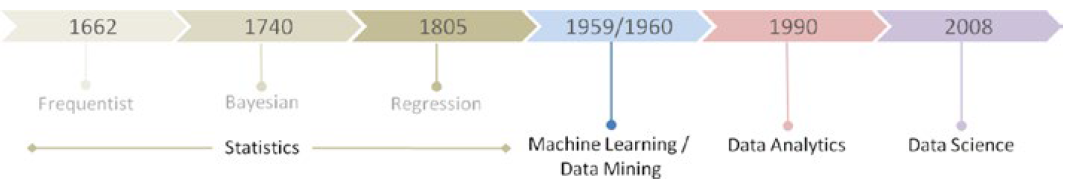
\includegraphics[width=\textwidth]{images/LearnFromDataEvolution.png}
\caption{Learn from data evolution \citep[S.~66]{swamynathan_mastering_2017}}
\label{fig:dataEvolution}
\centering
\end{figure}
\newline
Wie anfänglich erwähnt, sind alle genannten Begriffe miteinander verwandt. Das Gewinnen von Erkenntnissen aus Daten, um beispielsweise die Zukunft vorherzusagen, nennt sich Data Analysis. Werden die Daten aus verschiedensten Datenbanken oder Datawarehouses gewonnen, spricht man von Data Mining. Handelt es sich dabei noch um Informationen unterschiedlicher Struktur und große Datensätze, so befindet man sich im Bereich der Data Science. Der inhärente Erkenntnisgewinn dieser Verfahren kann von von menschlicher Seite kommen oder durch Machine Learning geschehen.\newline
Verdeutlicht wird dies durch Projekte wie Googles DeepMind\citep{deepmind_technologies_limited_deepmind_2017}, IBMs Watson\citep{international_business_machines_corporation_ibm_ibm_2017} oder Sprachassistenten wie Siri, Alexa und Bixby. Sie zeigen, dass großes Interesse an Machine Learning und Data Science herrscht. Deshalb haben sich auch ganze Berufsfelder wie "machine learning engineer", "data engineer" oder "data scientist"\citep[S.~1]{ramasubramanian_machine_2017} gebildet.



\section{Cloud-Dienste und SaaS}
Cloud Computing beschreibt "ein Modell, das es erlaubt bei Bedarf, jederzeit und überall bequem über ein Netz auf einen geteilten Pool von konfigurierbaren Rechnerressourcen (z. B. Netze, Server, Speichersysteme, Anwendungen und Dienste) zuzugreifen, die schnell und mit minimalem Managementaufwand oder geringer ServiceproviderInteraktion zur Verfügung gestellt werden können"\citep[S.~18]{appelrath_future_2014-1}. Innerhalb des Cloud Computing unterscheidet man weiterhin zwischen verschiedenen Cloud-Diensten (engl. cloud services). Nach \citep[S.~20]{appelrath_future_2014-1} differenziert man zwischen den Services in \ref{tab:CloudServices}.
\begin{table}[h]
\begin{tabular}{|p{5cm}|p{10cm}|}
\hline
\textbf{Diensttyp} & \textbf{Beschreibung}\\
\hhline{==}
Infrastructure as a Service (IaaS) & Virtuelle Hardware oder Infrastruktur, zum Beispiel Speicherplatz, Rechenleistung oder Netzwerkbandbreite\\
\hline
Platform as a Service (PaaS) & Programmierframeworks, Bibliotheken und Werkzeuge, um Anwendungen unter eigener Kontrolle auf
Cloud-Infrastrukturen bereitstellen zu können, ohne die zugrunde liegende Infrastruktur wie Netzwerk,
Server, Betriebssysteme oder Speicher managen oder kontrollieren zu müssen\\
\hline
Software as a Service (SaaS) & Vollständige Anwendungen, die auf Cloud-Infrastrukturen betrieben und beispielsweise über einen
Webbrowser aufrufbar sind, wobei Nutzer weder die zugrunde liegende Cloud-Infrastruktur noch
individuelle Anwendungseinstellungen (mit der möglichen Ausnahme der eingeschränkten Konfiguration
von Nutzereinstellungen) kontrollieren müssen und können\\
\hline
Mashup as a Service (MaaS) & Verknüpfung einzelner Software-Komponenten (unter anderem auch Cloud-Dienste) zu einem aggregierten
Cloud-Dienst\\
\hline
Business Process as a Service (BPaaS) & Konkrete Geschäftsanwendungen (beispielsweise CRM) als Verknüpfung einzelner Software-Komponenten
(standardisierte MaaS)\\
\hline
\end{tabular}
\caption{Cloud-Diensttypen}
\label{tab:CloudServices}
\end{table}
\citep[S.~23]{appelrath_future_2014-1} sprechen generell von "Cloud Computing als disruptiver Innovationsfaktor". An dieser Stelle wird besonders Software as a Service betrachtet. Dort stieg der Umsatz von 10,75 Mrd. USD im Jahr 2010 auf 38,57 Mrd. USD im Jahr 2016. Für die Zukunft (2020) wird sogar ein Umsatz von 75,73 Mrd. USD prognostiziert.\citep{gartner_umsatz_2017} Das ist eine Steigerung von über 700\% in nur 10 Jahren. Dies kann einerseits durch offensichtliche Vorteile, wie "höhere Stabilität und Planungssicherheit", der "Möglichkeit Anwender schnell ins System einzuführen" und "Erschließung neuer Kundengruppen"\citep{fraunhofer_vorteile_2010} erklärt werden, andererseits aber auch durch Tendenz der Softwarebranche hin zur serviceorientierten Architekturen (engl. service oriented atchitekture; SOA).\citep[S.~22]{appelrath_future_2014-1} Dieser Trend zu SaaS kann beobachtet werden, wenn reine Cloud-Anbieter wie Salesforce "klassische" Anbieter wie SAP den Rang als "Spitze des Weltmarkts der Software für Customer Relationship Management (CRM)"\citep{fritsch_salesforce.com_2013} ablaufen.\newline
Laut einer Studie von \citep{bitkom_welche_2017} greifen 23\% der befragten Unternehmen in Deutschland neben "Office Anwendungen aus der Cloud", "Security as a Service" und "Groupware" auf "Business Intelligence/Big Data"-Software aus der Cloud zurück. Zu dieser Kategorie gehört auch Azure Machine Learning (kurz: Azure ML) von Microsoft, welches zur Analyse in dieser Arbeit verwendet wird.

\chapter{Vorgehen und Ziele}\label{chapter:Vorgehen}
Nachdem in Kapitel \ref{chap:motivation} das Thema der Arbeit (\ref{sec:thema}) vorgestellt und die Motivation dahinter erläutert wurde (\ref{sec:cryptocurrency} bis \ref{sec:SaaS}), wird nun der restliche Aufbau vorgestellt.
Die nächsten vier Kapitel befassen sich mit den Grundlagen hinter der Arbeit (\textbf{Theorie}): 
\begin{itemize}
\item Kapitel \ref{sec:DataMiningFrameworks} geht auf Data Mining Frameworks ein. Dabei werden das Knowledge Discovery in Databases (KDD) process model (\ref{sec:kdd}) und der CRoss Industrial Standard Process for Data Mining (CRISP – DM (\ref{sec:crispdm}) betrachtet. Anschließend folgt eine Entscheidung für CRISP-DM in Punkt \ref{sec:crispdmdec}.
\item Daraufhin (Kapitel \ref{sec:MachineLearning}) folgen Erklärungen zu den Kategorien des Machine Learning: Supervised Learning (\ref{subsec:sl}), Unsupervised Learning (\ref{sec:us1}), Semi-supervised Learning (\ref{sec:ssl1}), Active Learning (\ref{sec:al1}) und Reinforcement Learning (\ref{sec:rl1}).
\item Genauere (technische) Details zu Kryptowährungen sind in Kapitel \ref{sec:cryptocurrency2} festgehalten. Hier sind Definitionen zu Begriffen zu finden, die später für die Analyse genutzt werden.
\item Den Abschluss des Theorieteils stellt die Allgemeine Beschreibung (\ref{sec:ab1}), der Aufbau und die Komponenten (\ref{sec:auK1}) von Microsoft Azure Machine Learning Studio in Kapitel \ref{sec:msmls} dar.
\end{itemize}
Im \textbf{Praxisteil} in Kapitel \ref{chap:praxis} werden
\begin{itemize}
\item zuerst Ziele und Projektressourcen festgelegt (\ref{sec:p1}).
\item Daraufhin werden Daten beschafft, beschrieben und untersucht (\ref{sec:p2}).
\item Nach ihrer Auswahl und Aufbereitung (\ref{sec:p3}) folgt
\item die Auswahl der Machine Learning Algorithmen, die Festlegung des Testdesigns, Durchführen des Machine Learnings und die Auflistung der Ergebnisse (\ref{sec:p4}).
\item Die Ergebnisbewertung, der Prozessrückblick und die nächsten Schritte (\ref{sec:p4}) stellen den Abschluss dar.
\end{itemize}
Das Schlusskapitel (\ref{chap:Bewertung}) bewertet die drei Kernelemente der Arbeit:
\begin{itemize}
\item das Azure Machine Learning Studio (\ref{sec:BeswertungAzure}),
\item das CRISP-DM Referenzmodell (\ref{sec:BeswertungCrisp}) und
\item die Ergebnisse des Machine Learning (\ref{sec:BewertungML}).
\end{itemize}
Das Hauptziel der Arbeit ist es, zu untersuchen, ob sich der Kurs von Kryptowährungen mit Hilfe von Machine Learning vorauszusagen lässt oder nicht.\newline
Für alle Teile sei angemerkt, dass die Fachliteratur fast ausschließlich in englischer Sprache verfügbar ist. In dieser Arbeit wird deshalb die Entscheidung getroffen, die Fachbegriffe nicht zu übersetzten. Auch die Prozessschritte und -artefakte (Outputs) des CRISP-DM-Referenzmodells sind davon betroffen. 


\chapter{Data Mining Frameworks}\label{sec:DataMiningFrameworks}
Wie in Abschnitt \ref{sec:DataMining} bereits erwähnt, haben sich um das Data Mining drei bekannte Frameworks entwickelt. Zwei davon (\gls{kdd} und \gls{crisp}) werden im Nachfolgenden genauer beschrieben. Danach wird eines der beiden für die Untersuchung in der Arbeit ausgewählt. Da der \gls{semma}-Process dem CRIPS-DM Referenzmodell einerseits sehr ähnelt und andererseits genau genommen "keine Data Mining Methodik, sondern eher eine logische Organisation" des Data Mining "tool set[s]"\citep[eigene Übersetzung]{enterpriseminer_sas_2012} ist, wird er hier ausgeklammert. 

\section{Knowledge Discovery in Databases (KDD) process model}\label{sec:kdd}
Die Bezeichnung Knowledge Discovery in Databases wurde hauptsächlich von \citep{fayyad_data_1996} geprägt. Sie beschreiben in ihrer Arbeit ein Problem, das in den 1990er Jahren aufkam. Wie auch heute noch, stieg damals die Masse der gespeicherten Daten rapide an. Die manuelle Auswertung dieser Datensätze erforderte mehr Arbeitskraft als vorhanden war. \citep[S.~38]{fayyad_data_1996} beschreiben es als "data overload". Deswegen versuchte man, die Prozesse zur Findung von Erkenntnissen zu automatisieren. Daraus hat sich ein Standardvorgehen entwickelt, das das KDD-Prozessmodell darstellt (siehe Abbildung \ref{fig:kddprocess}).
\begin{figure}[H]
\centering
\frame{
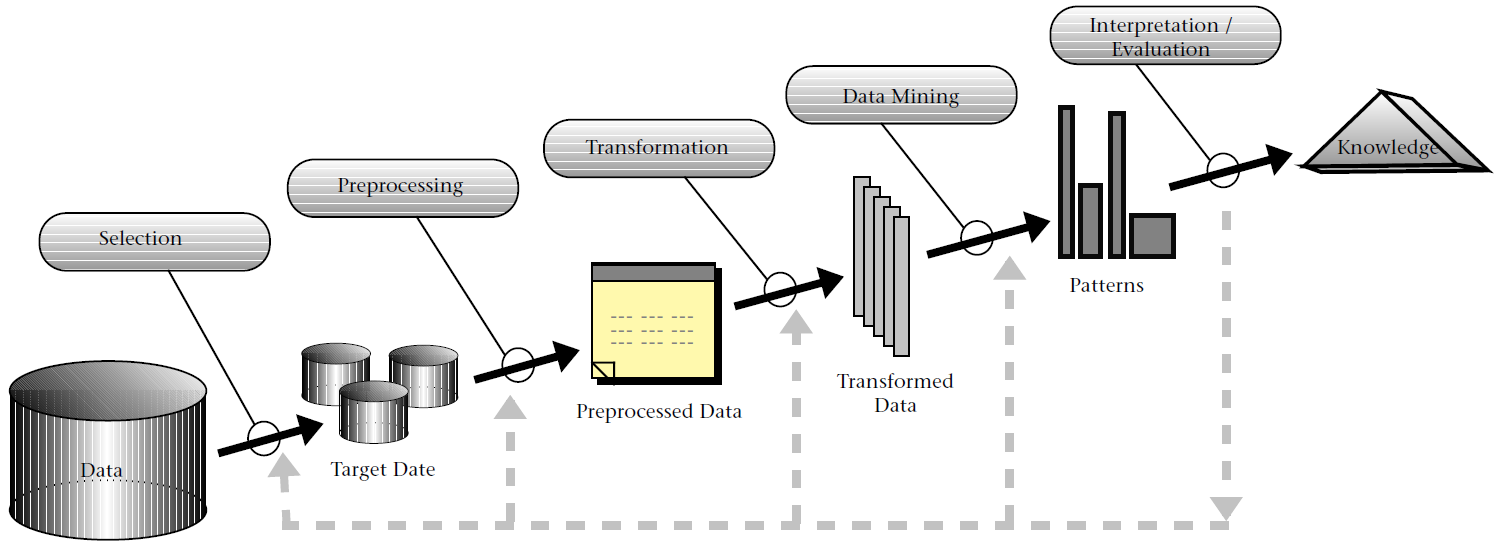
\includegraphics[width=\textwidth]{images/kddprocess}}
\caption{Ein Überblick über die Schritte des KDD Prozesses nach \citep[S.~41]{fayyad_data_1996}}
\label{fig:kddprocess}
\end{figure}

\subsection{Selection}
Bevor der erste eigentliche Schritt, die Selektion der Daten, erfolgen kann, ist es unabdingbar, ein "Verständnis für das Anwendungsgebiet zu entwickeln" \citep[S.~42; eigene Übersetzung]{fayyad_data_1996}. Dies inkludiert auch, Ziele zu setzen und Fragen zu formulieren, die durch das spätere Data Mining (Schritt \ref{subsubsec:DataMining}) beantwortet werden sollen. Ist das Verständnis vorhanden, kann ein "target data set"\citep[S.~42]{fayyad_data_1996} hergestellt werden. Dabei werden zuerst Daten aus unterschiedlichen - oft heterogenen - Quellen zusammengeführt und dann hinsichtlich des Ziels verdichtet \citep[S.~70]{swamynathan_mastering_2017}.

\subsection{Preprocessing}
Die verbleibende Teilmenge der ursprünglichen Daten muss nun gesäubert und für die nächsten Schritte vorbereitet werden. Dies ist notwendig, da unbereinigte Daten sowohl den Data Mining-Prozess verschlechtern (unverlässliche oder falsche Ergebnisse), als auch die Zeit für das Mining deutlich verlängern können \citep[S.~70]{swamynathan_mastering_2017}.
Um die Qualität der Daten und des Mining zu verbessern, werden unter anderem folgende Aspekte betrachtet\multicitep{fayyad_data_1996, S.~42; swamynathan_mastering_2017, S.~70}:

\subsubsection{Outliner treatment}
Ein Ausreißer (engl. outliner) kann beispielsweise ein "Extremer Wert in einer Variablen" oder ein "Extremer Wert des Residuums bei einer sinnvollen Regression"\citep[S.~25; Teil 5b]{hertle_datenanalyse_2016} sein. Ein Vorgehen für Ausreißer kann folgendermaßen aussehen (nach \citep[S.~25; Teil 5b]{hertle_datenanalyse_2016}):
\begin{enumerate}
\item Identifizieren der Ausreißer (evtl. durch eine erste Regression)
\item Interpretation im Sachzusammenhang (Messfehler oder wichtiger Teil der Population)
\item Entscheidung, ob man eine Regression der Daten mit oder ohne diese Ausreißer haben möchte
\item In der Darstellung der Ergebnisse auf die Ausreißer explizit eingehen und Vorgehen erläutern
\end{enumerate}

\subsubsection{Noise removal}
Auch in einem Datensatz, der auf Ausreißer untersucht wurde, befinden sich immer noch unbekannte, unvollständige, falsche und fehlende Werte ("attribute noise"). Zusätzlich können Datenklassen falsch gekennzeichnet sein ("class noise"). Ist ein Datensatz von diesen Problemen betroffen, spricht man von "noisy data". Auf die Lösung dieses Problems wird an dieser Stelle nicht weiter eingegangen. 

\subsubsection{Identifying duplicated values}
Wie oben angesprochen, wird der zu analysierende Regression ohne Datensatz aus mehreren Quellen zusammengeführt. Durch diesen Schritt können Datensätze doppelt (oder noch öfter) vorkommen. Das wird deutlich, wenn man folgendes Beispiel betrachtet: \par
Über eine Kundenkarte werden Daten von Kunden eines Supermarktes je Filiale gespeichert. Bei einer überregionalen Kundenanalyse tauchen Kunden mehrfach auf, die in verschiedenen Filialen eingekauft haben. Hier ist anzumerken, dass doppelte Werte nicht zwangsläufig gelöscht werden müssen, sie sollten jedoch bei der Analyse bedacht werden.

\subsubsection{Check for inconsistency}
Je größer ein Datensatz ist, umso wahrscheinlicher enthält er Inkonsistenzen. Dies wird ebenfalls durch die Fusion von mehreren Quellen verstärkt (Beispiel: unterschiedliches Alter für einen Kundenstammsatz). Auch hier muss geprüft werden, wie mit diesen Werten umzugehen ist. Eventuell können Regeln festgelegt werden wie 'immer der neuste Datenpunk ist der richtige'.

\subsubsection{Time series and changes}
Der letzte Punkt, der beim Preprocessing betrachtet werden muss, ist der Zusammenhang der Daten mit dem Erfassungszeitpunkt. So können sich im Laufe der Zeit die Messmethodik (z.B. andere Sensoren), die Messgenauigkeit (z.B. bessere Sensoren) oder die Abstände der Messungen verändern. Das wiederum kann zu ungleich verteilten Datensätzen oder inkonsistenter Genauigkeit führen.

\subsection{Transformation}
Der letzte Schritt vor dem eigentlichen Data Mining ist die Transformation. In diesem Prozessschritt geht es darum, "mit Dimensionsreduktions- oder -transformationsmethoden die effektive Anzahl an Variablen [...] zu reduzieren"\citep[S.~42; eigene Übersetzung]{fayyad_data_1996}. Dies geschieht beispielsweise durch das Identifizieren und Eliminieren invarianter Variablen. Ebenfalls wird versucht, solche Variablen zu finden, die mehrere Andere repräsentieren. Anschaulich dargestellt an einem Beispiel:\par
\begin{table}[H] \centering
\begin{tabular}{|r|r|r|r|r|r|r|}
  \hline
 & \textbf{Person} & \textbf{Studium} & \textbf{ErfahrungExtern} & \textbf{ErfahrungIntern} & \textbf{Alter} & \textbf{Gehalt} \\ 
\hhline{=======}
1 &   1 &   6 &   1 &   4 &  24 & 46450 \\ 
  2 &   2 &  18 &  30 &  15 &  55 & 85150 \\ 
  3 &   3 &  11 &   7 &   7 &  31 & 55900 \\ 
  4 &   4 &  11 &  15 &   8 &  36 & 63650 \\ 
  5 &   5 &  10 &   1 &  16 &  33 & 59050 \\ 
  6 &   6 &   6 &  25 &   6 &  38 & 68750 \\ 
  7 &   7 &  10 &  20 &  20 &  50 & 79000 \\ 
  8 &   8 &   7 &   0 &   1 &  23 & 43050 \\ 
   \hline
\end{tabular}
\caption{Einfacher Datensatz mit Berufserfahrung und Gehalt}
\label{tab:Beispiel_Berufserfahrung_R_output_simpleData}
\end{table}
Tabelle \ref{tab:Beispiel_Berufserfahrung_R_output_simpleData} zeigt einen einfachen Datensatz, in dem die Mitarbeiter einer Firma und die zugehörigen Gehälter festgehalten sind. "Studium" beschreibt die Anzahl der Halbjahre im Studium. Analog dazu "ErfahrungExtern" und "ErfahrungIntern" die Berufserfahrung in Halbjahren außerhalb und innerhalb der Firma. Zusätzlich ist das Alter der Personen gegeben.\par
Führt man eine lineare Regression (Listing \ref{list:Regression1}) für den Datensatz durch (mit Studium, ErfahrungExtern, ErfahrungIntern, Alter als unabhängige und Gehalt als abhängige Variablen), ergibt sich das Ergebnis in Tabelle \ref{tab:Regression1:output}.

\lstinputlisting[caption=Regression mit allen Faktoren,label=list:Regression1]{../R/Beispiel_Berufserfahrung/Regression1.R}

\begin{table}[H] \centering
\begin{tabular}{|rrrrr|}
  \hline
 & \textbf{Estimate} & \textbf{Std. Error} & \textbf{t value} & \textbf{Pr($>$||)} \\ 
  \hhline{=====}
(Intercept) & 40000 & 1.415e-11 & 2.828e+15 & <2e-16 *** \\ 
  Studium & 300 & 5.167e-13 & 5.807e+14 & <2e-16 *** \\ 
  ErfahrungExtern & 850 & 4.821e-13 & 1.763e+15  & <2e-16 *** \\ 
  ErfahrungIntern & 950 & 6.308e-13 & 1.506e+15 & <2e-16 *** \\ 
  Alter & 2.010e-13 & 8.103e-13 & 2.480e-01 & 0.82 \\ 
  \hhline{=====}
  \multicolumn{4}{|l|}{Adjusted R-squared} & \multicolumn{1}{l|}{1}\\
\hline
\end{tabular}
\caption{Output der Regression mit allen Variablen}
\label{tab:Regression1:output}
\end{table}

Ohne weiter auf die genauen Bezeichnung einzugehen, gibt die Sternnotation von R an, dass die unabhängigen Variablen Studium, ErfahrungIntern und ErfahrungExtern signifikant sind (drei *), das Alter hingegen nicht (kein *). Die Regression hat ein adjustiertes Bestimmtheitsmaß (\gls{rs}; engl. adjusted R-squared) von 1. Das Bedeutet, dass das Gehalt vollständig durch die gegebenen Variablen erklärt werden kann (dies wird in der Realität jedoch nie erreicht).

\lstinputlisting[caption=Regression ohne Alter,label=list:Regression2]{../R/Beispiel_Berufserfahrung/Regression2.R}
\begin{table}[H] \centering
\begin{tabular}{|rrrrr|}
\hline
 & \textbf{Estimate} & \textbf{Std. Error} & \textbf{t value} & \textbf{Pr($>$||)} \\
  \hhline{=====}
(Intercept) & 40000 & 2.393e-12 & 1.671e+16 & <2e-16 *** \\ 
  Studium & 300 & 2.948e-13 & 1.018e+15 & <2e-16 *** \\ 
  ErfahrungExtern & 850 & 8.948e-14 & 9.500e+15 & <2e-16 *** \\ 
  ErfahrungIntern & 950 & 1.642e-13 & 5.787e+15.75 & <2e-16 *** \\ 
  \hhline{=====}
  \multicolumn{4}{|l|}{Adjusted R-squared} & \multicolumn{1}{l|}{1}\\
\hline
\end{tabular}
\caption{Output der Regression ohne die Variable 'Alter'}
\label{tab:Regression2:output}
\end{table}
Führt man die Regression nun ohne die Variable 'Alter' durch (Listing \ref{list:Regression2} und Tabelle \ref{tab:Regression2:output}) bleibt $R^2$ gleich. Der Datensatz wurde also bereits um eine Variable reduziert, ohne das Ergebnis der Regression zu verschlechtern.\par
Betrachtet man die Faktoren ErfahrungExtern und ErfahrungIntern, so fällt auf, dass sie einen ähnlichen Einfluss auf das Gehalt erzielen (850 und 950). 
\lstinputlisting[caption=Regression mit zusammengefassten Werten,label=list:Regression3]{../R/Beispiel_Berufserfahrung/Regression3.R}
Fasst man beide Variablen zusammen (Listing \ref{list:Regression3}), zeigt sich im Ergebnis (Tabelle \ref{tab:Regression3:output}), dass $R^2$ bei 0,9988 liegt. Die Güte der Regression hat sich also nur minimal verschlechtert.
\begin{table}[H] \centering
\begin{tabular}{|rrrrr|}
  \hline
 & \textbf{Estimate} & \textbf{Std. Error} & \textbf{t value} & \textbf{Pr($>$||)} \\
  \hhline{=====}
(Intercept) & 40107.10 & 528.87 & 75.83 & 7.55e-09 *** \\
ErfahrungGesamt & 876.69 & 15.86 & 55.26 & 3.67e-08 ***\\ 
Studium & 327.17 & 64.27 & 5.09 & 0.0038 **\\ 
  \hhline{=====}
  \multicolumn{4}{|l|}{Adjusted R-squared} & \multicolumn{1}{l|}{0.9988}\\
\hline
\end{tabular}
\caption{Output der Regression mit zusammengefassten Werten}
\label{tab:Regression3:output}
\end{table}
Zusammenfassend lässt sich für dieses Beispiel sagen, dass die Variablen im Datensatz um die Hälfte reduziert wurden, ohne die Aussagekraft deutlich zu verschlechtern. In einem realen Datensatz ist diese Arbeit zwar nicht so trivial und offensichtlich, jedoch gelten die gleichen Prinzipien.\par
Nach \citep[S.~71; veränderte Version]{swamynathan_mastering_2017} gibt es zur Transformation folgende Möglichkeiten:
\begin{itemize}
\item Smoothing (binning, clustering, regression, etc.)
\item Aggregation (im Beispiel: das Zusammenfassen der Berufserfahrung)
\item Generalization (Ersetzen von primitiven Datenobjekten durch höherstufige Konzepte)
\item Normalization (min-max-scaling oder z-score)
\item Feature construction aus bereits bestehenden Attributen durch Techniken wie die Hauptkomponentenanalyse (engl. principal components analysis; \gls{pca}), Multidimensional scaling (MDS) oder Locally-linear embedding (LLE)
\item Compression (zum Beispiel wavelets, PCA, clustering etc.)
\item andere Datenreduzierungstechniken bei denen das Datenvolumen sinkt, ohne die Integrität der Originaldaten zu verletzten
\end{itemize}


\subsection{Data Mining}\label{subsubsec:DataMining}
Ist der Datensatz präpariert, so findet das eigentliche Data Mining statt. Dabei muss sich der Anwender für eine oder auch mehrere Methoden für das Mining entscheiden, um die anfänglichen Ziele zu erreichen und die Fragestellungen zu beantworten. Zur Auswahl stehen beispielsweise\multicitep{fayyad_data_1996, S.~42; swamynathan_mastering_2017, S.~71}:
\begin{itemize}
\item zusammenfassende und beschreibende Methoden: Mittelwert (arithmetisches Mittel), Median, Modus, Standardabweichung, Klassen-und Konzeptbeschreibungen, grafische Plots,
\item Vorhersagende Modelle (engl. predictive models): Klassifikationen und Regressionen und
\item Cluster-Analysen.
\end{itemize}
Eine genauere Beschreibung der Methoden (und der zugehörigen Algorithmen) im Kontext des Machine Learning befindet sich in Kapitel \ref{sec:MachineLearning}. Je nach Beschaffenheit der zugrundeliegenden Daten und der gewählten Methode, muss ein passender Algorithmus gewählt und dieser korrekt parametrisiert werden. Zum Data Mining gehört auch, Hypothesen zu formulieren und das Ergebnis im Auge zu behalten: Ist der Endnutzer der Analyse an einem vorhersagenden Model interessiert (zum Beispiel für Wartungsarbeiten) oder an einem Jetzt-bezogenen (zum Beispiel für eine strategische Ausrichtung nach den aktuellen Kundensegmenten)?\par
Anschließend erfolgt das (automatische) Mining der Daten. Je besser die vorhergehenden Schritte durchgeführt wurden, desto potenter ist das Ergebnis \citep[S.~42]{fayyad_data_1996}. Aus diesem Grund ist es jederzeit möglich, zu einem vorangegangen Prozessschritt zurückzukehren, um neu erlangte Einsichten einfließen zu lassen (siehe zurückspringender gestrichelter, grauer Pfeil in Abbildung \ref{fig:kddprocess}).

\subsection{Interpretation/Evaluation}
Zuletzt werden die gefundenen Muster und trainierten Modelle interpretiert. Ein Muster macht Aussagen über jeden Datenpunkt im betrachteten Raum. Ein Beispiel bei einem einfachen linearen \gls{model}: $$y = m \times x + t$$
Zu obigem Fall: $$Gehalt = Studium \times 327,17 + ErfahrungGesamt \times 876,69 + 40107,10$$ Ein Muster (engl. pattern) beschreibt dagegen nur eine kleine "lokale Struktur", die "nur über einen begrenzten Bereich" Aussagen macht \citep[S.~71; eigene Übersetzung]{swamynathan_mastering_2017}. Im Fall des linearen Model, wäre es eine bestimmte Gleichung, zum Beispiel $$y = 2 \times x + 5$$ oder $$ 6 \times 327,17 + 5 \times 876,69 + 40107,10 =  46453,57$$\citep{kraker_towards_2013}. "Fayyad et al. benutzt patterns und models synonym" \citep{kraker_towards_2013}.\par
Das Interpretieren der Ergebnisse beinhaltet ebenfalls das Zusammenfassen der Erkenntnisse und gegebenenfalls das Visualisieren \citep[S.~71]{swamynathan_mastering_2017}. Als Evaluieren wird das Eingliedern der Resultate in andere Systeme (zur Weiterverarbeitung oder Verbreitung), das Prüfen auf (und Lösen von) Konflikten mit anderen Untersuchungen und nicht zuletzt das Dokumentieren der Befunde bezeichnet \citep[S.~42]{fayyad_data_1996}. \par
An dieser Stelle sei erneut angemerkt, dass das erste Ergebnis des KDD-Prozesses nicht das Endergebnis sein muss. Es kann durchaus viele Iterationen geben, die auch "loops between any two steps" beinhalten können \citep[S.~42]{fayyad_data_1996}.

\section{CRoss Industrial Standard Process for Data Mining (CRISP – DM)}\label{sec:crispdm}
Bei CRoss Industrial Standard Process for Data Mining handelt es sich - wie bei KDD - um ein Referenzmodell für Data Mining. Das Modell wurde von einem 1996 gegründeten Konsortium aus "Daimler-Benz (now DaimlerChrysler), Integral Solutions Ltd. (ISL) [jetzt SPSS], NCR, and OHRA"\citep[S.~13]{shearer_crisp-dm_2000} erarbeitet. Die Version 1.0 wurde 2000 vorgestellt \citep[S.~13]{shearer_crisp-dm_2000}. In Umfragen (1999, 2002, 2004, 2007) wird das Modell als führend in Bereich von "data mining/predictive analytics projects"\citep[S.~72]{swamynathan_mastering_2017} bezeichnet. Das Modell ist "nicht-proprietär, dokumentiert und frei verfügbar"\citep[S.~13; eigene Übersetzung]{shearer_crisp-dm_2000}. Es ist ebenfalls in vielen Bereichen nutzbar, da es weder industriesektor-, werkzeugs- noch anwendungsspezifisch ist. Grundsätzlich bekräftigt das Modell best practices und soll zu besseren und schnelleren Ergebnissen führen \citep[S.~13; eigene Übersetzung]{shearer_crisp-dm_2000}. 

\begin{figure}[H]
\centering
\frame{
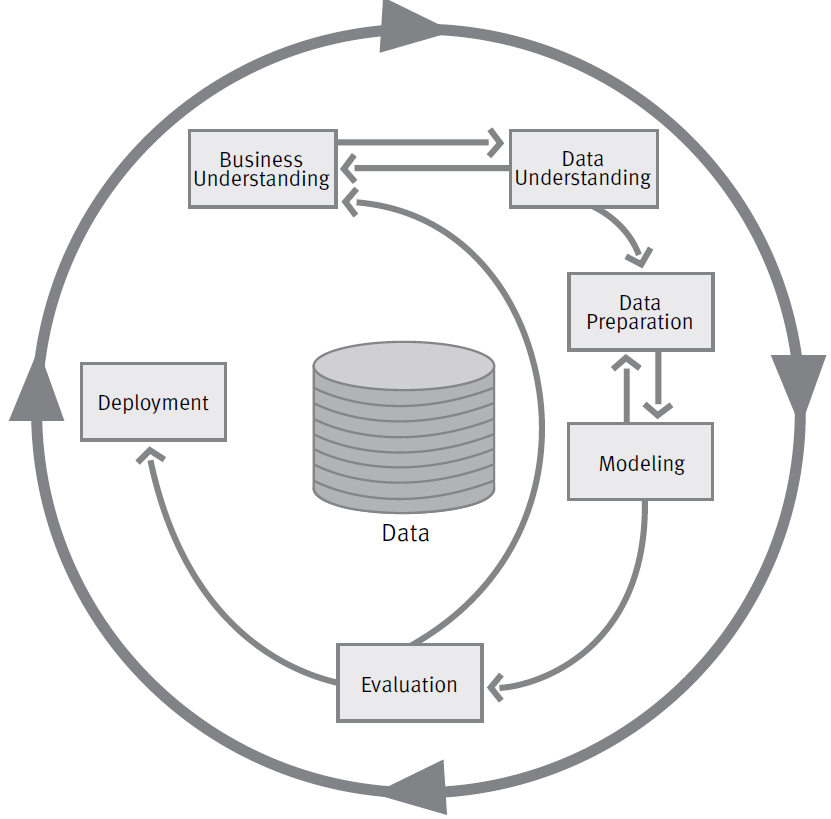
\includegraphics[width=12cm]{images/CRISP_DM}}
\caption{Phasen des CRISP-DM Referenzmodells nach \citep[S.~10]{chapman_crisp-dm_2000}}
\label{fig:CRISP_DM}
\end{figure}

Wie in Abbildung \ref{fig:CRISP_DM} zu sehen ist, umfasst das Referenzmodell sechs Phasen. Genau wie beim KDD-Prozessmodell handelt es sich nicht um ein lineares Modell, sondern um eines, das Rückschritte und Iterationen erlaubt. Im Nachfolgenden wird zuerst immer ein Prozessschritt kurz vorgestellt und darunter detaillierter betrachtet. Als Referenz dient unter anderem Abbildung \ref{fig:CRISP_DM_detailed}, die den Output der einzelnen Schritte zeigt.

\begin{figure}[H]
\centering
\frame{
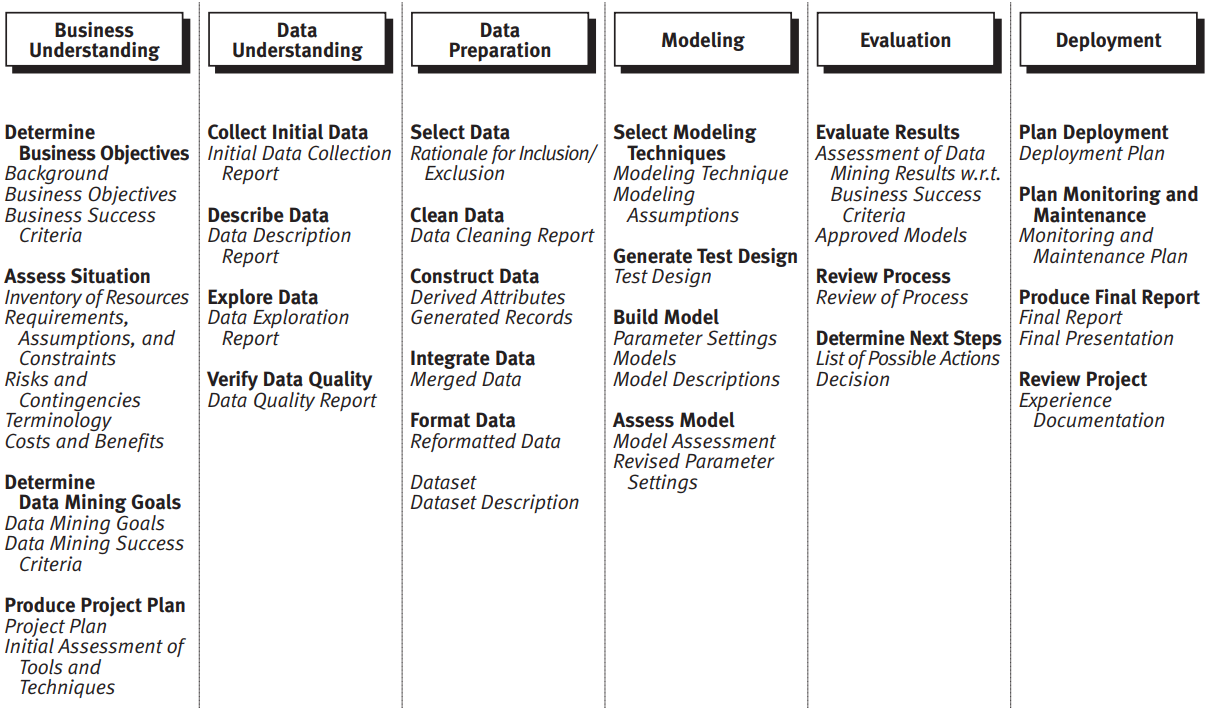
\includegraphics[width=\textwidth]{images/crisp_dm_detailed}}
\caption{Generische Aufgaben (\textbf{fett}) und Output (\textit{kursiv}) des CRISP-DM Referenzmodells \citep[S.~12]{chapman_crisp-dm_2000}}
\label{fig:CRISP_DM_detailed}
\end{figure}

\subsection{Business Understanding}
Die erste und vielleicht wichtigste Phase\citep[S.~14]{shearer_crisp-dm_2000} des CRISP-DM Prozesses ist das "Business Understanding", oder auch "Research Understanding"\citep[Punkt 1.4.1.1]{larose_discovering_2014}. Die Aufgabe dieser Phase ist es, die "Ziele und Erwartungen"\citep[S.~73]{swamynathan_mastering_2017} des Projektes zu verstehen, dieses "Wissen in eine Machine Learning Problem Definition zu übersetzen" und schließlich einen "Vorläufigen Plan"\citep[S.~14]{shearer_crisp-dm_2000} aufzustellen: 
\subsubsection{Determine the Business Objectives}
Dieser Teilschritt soll hauptsächlich die Frage beantworten, warum die Analyse durchgeführt wird. Dies hat direkten Einfluss auf die Ziele des Projekts und soll verhindern, dass "viel Aufwand für das Finden von richtigen Antworten auf falsche Fragen"\citep[S.~14]{chapman_crisp-dm_2000} verschwendet wird.
\subsubsection{Assess the Situation}
Um das Ziel der Analyse so genau wie möglich zu treffen, muss genau nachgeforscht werden, welche Ressourcen verfügbar sind, welchen Zwängen und Grenzen die Analyse unterlegen ist und unter welchen Annahmen sie stattfindet \citep[S.~14]{chapman_crisp-dm_2000}. Vereinfacht lässt sich sagen, dass hier die Fragen aus dem vorhergehenden Schritt detaillierter betrachtet werden.
\subsubsection{Determine the Data Mining Goals}
Die gefundenen Ziele sind meist in Geschäftssprache formuliert. Für die Analyse müssen die Ziele jedoch im Terminus technicus des Data Mining formuliert sein. Ein Beispiel dazu ist die Übersetzung von "Increase catalog sales to existing customers" in "Predict how many widgets a customer will buy, given their purchases over the
past three years, demographic information (age, salary, city, etc.), and the price of the item."\citep[S.~16]{chapman_crisp-dm_2000}
\subsubsection{Produce a Project Plan}
Der Projektplan (engl. Project Plan) liefert einen konkreten Plan, wie die gesetzten Ziele zu erreichen sind. Nach \citep[S.~15]{shearer_crisp-dm_2000} beinhaltet er:
\begin{itemize}
\item Die Schritte, die nacheinander durchzuführen sind.
\item Eine Timeline für die Durchführung.
\item Eine Auflistung potentieller Risiken im Projektverlauf.
\item Eine Aufstellung der zu nutzenden Werkzeuge und Techniken \citep[S.~16]{chapman_crisp-dm_2000}
\end{itemize}


\subsection{Data Understanding}
In der vorhergegangenen Phase wurde festgelegt, welche Daten zum Erreichen der Ziele benötigt werden. Nun werden diese Daten gesammelt und untersucht. Im Fokus der Untersuchung liegt dabei\citep[S.~73]{swamynathan_mastering_2017}
\begin{itemize}
\item Datenlücken zu  finden,
\item die Relevanz der erfassten Daten (hinsichtlich der Ziele) zu klären,
\item die allgemeine Datenqualität festzustellen und
\item "erste Einblicke in Daten" zu erhalten, um "geeignete Hypothesen"\citep[S.~73; eigene Übersetzung]{swamynathan_mastering_2017} zu formulieren.
\end{itemize}
Im Zuge dessen können auch bereits "subsets" isoliert werden, die "actionable patters"\citep[Punkt 1.4.1.2.d]{larose_discovering_2014} (etwa: verfolgbare Muster) enthalten könnten. Mit jedem Fortschritt in dieser Phase ist es eventuell nötig, das Ergebnis der Business Understanding-Phase zu adjustieren. Durch dieses Vorgehen entsteht ein iterativer Prozess \citep[S.~73]{swamynathan_mastering_2017}. Larose empfiehlt den Einsatz von explorativer Datenanalyse (siehe Abschnitt \ref{sec:DataMining}) \citep[Punkt 1.4.1.2.b]{larose_discovering_2014}. 


\subsubsection{Collect the Initial Data}
Die Hauptaufgabe dieses ersten Schrittes ist es, die benötigten Daten zu beziehen. Dabei kann entweder der direkte Zugriff auf die Daten gemeint sein oder nur das Erhalten der Zugangsinformationen. Eventuell werden die Datensätze gleich in Systeme oder Werkzeuge geladen, die zur späteren Weiterverarbeitung genutzt werden. Die Integration inhomogener Daten (unterschiedliche Strukturen/Formate etc.) kann bereits hier erfolgen oder in der Data Preparation (siehe Punkt \ref{subsubsec:DataPreperation}). \citep[S.~18]{chapman_crisp-dm_2000}

Sollten in diesem Schritt Probleme auftauchen, müssen sie - wenn möglich mit Lösung - gut dokumentiert werden, um den Projektverlauf reproduzierbar zu gestalten. Ein Beispiel können lange Antwortzeiten einiger Datenquellen sein \citep[S.~15]{shearer_crisp-dm_2000}.

\subsubsection{Describe the Data}
Im Schritt "Describe the Data" werden die beschafften Daten oberflächlich beschrieben \citep[S.~18]{chapman_crisp-dm_2000}. Dabei wird unter anderem auf 
\begin{itemize}
\item das Format der Daten,
\item die Größe des Datensatzes,
\item die Anzahl der Beobachtungen und Einträge in den Daten und 
\item die Beschaffenheit der Einträge
\end{itemize}
geachtet. Dabei soll einerseits die Frage geklärt werden, ob die vorhandenen Daten alle relevanten Informationen für die Ziele des Data Mining enthalten. Andererseits wird das Verständnis der Daten geschärft \citep[S.~15]{shearer_crisp-dm_2000}.

Anhand des nachfolgenden Beispiels (Datensatz von \citep[Case Lasagne Test.xlsx]{hertle_datenanalyse_2016}) werden die Schritte "Collect the Initial Data" und "Describe the Data" kurz visualisiert. Zuerst werden die Daten eingelesen (Listing \ref{list:LasagneHead}) und anschließend oberflächlich betrachtet.
\lstinputlisting[caption=Einlesen aller Daten und Betrachten des "Kopfes" ,label=list:LasagneHead]{../R/Beispiel_Head_Lasagne/head_lasagne.R}
Aus Tabelle \ref{tab:LasagneHead:output} kann abgelesen werden, dass es sich um einen Datensatz mit 12 Variablen handelt. 
\begin{table}[H] \centering
\centering
\begin{tabular}{|p{1.2cm}|p{0.9cm}|p{2.1cm}|p{1.8cm}|p{1.9cm}|p{3.6cm}|p{1.9cm}|}
  \hline
\textbf{Person} & \textbf{Alter} & \textbf{Einkommen} & \textbf{Angestellt} & \textbf{Wert.Auto} & \textbf{Umsatz.Kreditkarte} & \textbf{Geschlecht} \\ 
  \hhline{=======}
1 &  48 &  91700 & nein & 2190 & 3510 & m\\ 
2 &  33 &  40740 & nein & 2110 & 740& w\\ 
3 &  51 &  45080 & ja & 5140 & 910 & m\\ 
4 &  56 &  26600 & nein & 700 & 1620 & w\\ 
5 &  28 &  113960 & ja & 26620 & 600 & m\\ 
6 &  51 &  102200 & ja & 24520 & 950 & w\\ 
\hline
\end{tabular}
\begin{tabular}{|p{1.4cm}|p{2.3cm}|p{2.2cm}|p{5.8cm}|p{3cm}|}
  \hline
\textbf{Gewicht} & \textbf{alleinstehend} & \textbf{Wohnung} & \textbf{Supermarkt.besuche.pro.Monat} & \textbf{Lasagne.probiert}\\ 
  \hhline{=====}
65 & nein & Haus &   7 & nein\\ 
75 & nein & Wohnung &   4 & ja\\ 
70 & nein & Wohnung &   1 & nein\\ 
91 & nein & Haus &   3 & nein\\ 
81 & nein & Appartement &   3 & ja\\ 
65 & nein & Wohnung &   2 & nein\\ 
   \hline
\end{tabular}
\caption{Aufruf des head()-Befehls zum Betrachten der Daten}
\label{tab:LasagneHead:output}
\end{table}
Ebenfalls entnommen werden kann, dass es sich um demographische Angaben über Personen handelt. Zusätzlich wurde zu jeder Person erfasst ob sie Lasagne probiert hat. In Abbildung \ref{fig:Lasagne_RStudio} wird der Datensatz schließlich in RStudio betrachtet.
\begin{figure}[H]
\centering
\frame{
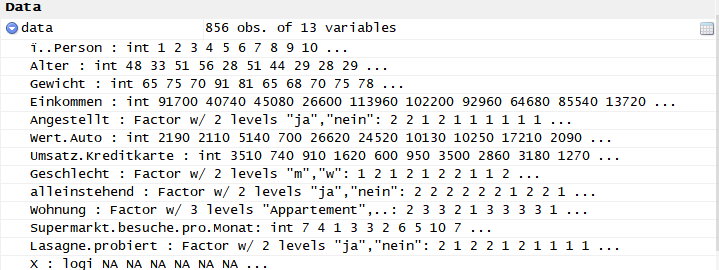
\includegraphics[width=\textwidth]{images/Lasagne_data}}
\caption{Betrachten der Datentypen des Datensatzes in RStudio}
\label{fig:Lasagne_RStudio}
\end{figure}
Zu sehen ist hier, dass es sich um einen Datensatz mit 13 Variablen und 856 Beobachtungen handelt (hier scheint ein falscher Zeichensatz vorzuliegen, da eine zusätzliche leere Spalte "X" angezeigt wird). Zusätzlich können die vorgeschlagenen Datentypen von R betrachtet werden. Bei den meisten Spalten handelt es sich um Ganzzahlen (int) oder Faktoren (manchmal auch als Enums bezeichnet) wie m/w für männlich und weiblich.

\subsubsection{Explore the Data}
Ist die grobe Sichtung der Daten abgeschlossen, wird enger an der Fragestellung des Data Mining gearbeitet. Dazu werden "Abfrage-, Visualisierungs- und Reporting[-Techniken]"\citep[S.~16; eigene Übersetzung]{shearer_crisp-dm_2000} eingesetzt. Um der Antwort auf die ursprüngliche Fragestellung näher zu kommen oder die Fragestellung zu verfeinern, werden beispielsweise folgende Eigenschaften betrachtet \citep[S.~18; eigene Übersetzung]{chapman_crisp-dm_2000}:
\begin{itemize}
\item Die Verteilung der Schlüsselattribute (zum Beispiel der Zielvariablen bei einer Vorhersage).
\item Die Beziehungen zwischen Wertepaaren oder kleinen Attributgruppen.
\item Die Ergebnisse einfacher Aggregationen.
\item Die Beschaffenheit von aussagekräftigen Teilgruppen von Werten.
\item Die Ergebnisse einfacher statistischer Analysen.
\end{itemize}

\subsubsection{Verify Data Quality}
Der letzte Schritt der zweiten Phase evaluiert die Qualität der Daten. \citep[S.19]{chapman_crisp-dm_2000} nutzen die Zielfragen: 
\begin{itemize}
\item "Is the data complete (does it cover all the cases required)?"
\item "Is it correct, or does it contain errors and, if there are errors, how common are they?"
\item "Are there missing values in the data?"
\item "If so, how are they represented, where do they occur, and how common
are they?"
\end{itemize}
\citep[S.~16]{shearer_crisp-dm_2000} empfiehlt zusätzlich noch, zu prüfen, ob die Werte plausibel sind, wie die Schreibweisen sind, ob Attribute mit unterschiedlichen Werten aber gleicher Bedeutung vorhanden sind und schließlich ob es einen "conflict with common sense", wie "teenagers with high income"\citep[S.~16]{shearer_crisp-dm_2000} gibt. 
\subsection{Data Preparation}\label{subsubsec:DataPreperation}
In der aufwendigsten Phase des ganzen Prozesses (siehe Abbildung \ref{fig:CRISP_DM_percent}) wird das "final data set"\multicitep{larose_discovering_2014, Punkt 1.4.1.3.a; shearer_crisp-dm_2000, S.~16} erzeugt. Dies geschieht durch\citep[S.~73]{swamynathan_mastering_2017}
\begin{itemize}
\item generelle Transformationen,
\item Füllen der Datenlücken, die in vorangegangenen Schritten aufgedeckt wurden,
\item Befassen mit fehlenden Werten,
\item Herausarbeiten, welche Features des Datensatzes die größte Relevanz haben und welche neuen Features sinnvoll wären.
\end{itemize}
Wie bereits erwähnt, handelt es sich nicht nur um die Phase, die den meisten Aufwand erfordert, sondern auch um die, von der die Genauigkeit des Endresultates zu großen Stücken abhängt \citep[S.~73]{swamynathan_mastering_2017}.

\begin{figure}[H]
\centering
\frame{
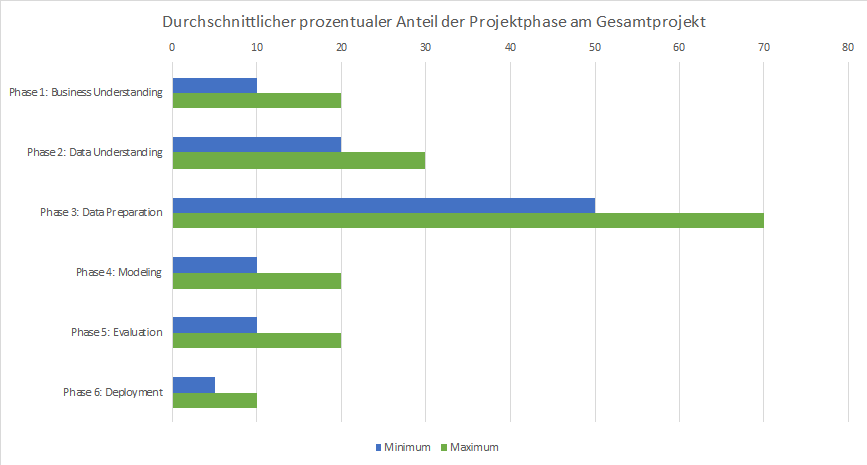
\includegraphics[width=\textwidth]{images/ProjektphasenInProzent_DRISP_DM}}
\caption{Durchschnittlicher prozentualer Anteil der CRISP-DM-Projektphase am Gesamtprojekt nach \citep[S.~15; eigene Darstellung]{shearer_crisp-dm_2000}}
\label{fig:CRISP_DM_percent}
\end{figure}

\subsubsection{Select Data}
Genauer wird dabei im ersten Schritt ausgewählt, welche Daten Teil der Analyse bleiben und welche exkludiert werden. Kriterien sind dabei, die Relevanz hinsichtlich der Ziele, die Qualität der Daten und technische Grenzen\citep[S.~16]{shearer_crisp-dm_2000} (wie "data volume or data types"\citep[S.~21]{chapman_crisp-dm_2000}). Zusätzlich kann überlegt werden, ob einige Attribute wichtiger sind als andere. So kann beispielsweise bei einer landesweiten Kundenanalyse die Postleitzahl der Kunden ausreichen und Straße und Hausnummer vernachlässigt werden \citep[S.~16]{shearer_crisp-dm_2000}. Chapman und seine Kollegen merken an, dass diese Phase sowohl "attributes (columns)", als auch "records (rows)" umfasst \citep[S.21]{chapman_crisp-dm_2000}. Wie bereits in den vorhergehenden Schritten muss auch hier erklärt werden, warum Entscheidungen getroffen wurden und eine Dokumentation angefertigt werden \citep[S.~16]{shearer_crisp-dm_2000}.

\subsubsection{Clean Data}
Im Schritt "Verify Data Quality" wurde herausgearbeitet, wie die Qualität der Daten ist und wie mängelbehaftet sie sind. Jetzt werden Maßnahmen dagegen ergriffen. Neben trivialen Vorgehen wie "Auswahl von reinen Untermengen" oder "Einfügen von passenden Standardwerten" können "anspruchsvollere Techniken wie das Schätzen von fehlenden Werten"\citep[S.21; eigene Übersetzung]{chapman_crisp-dm_2000} zum Zuge kommen.

\subsubsection{Construct Data}
Die gereinigten Daten sind noch nicht fertig für die Modeling-Phase. Manchmal ist es notwendig, einem Datensatz neue Zeilen hinzuzufügen. Betrachtet man wieder eine Kundenanalyse, so ist es vielleicht nötig, für einen Kunden, der in einem Quartal keinen Einkauf getätigt hat, einen leeren Einkauf (null Euro) anzulegen, falls der eingesetzte Algorithmus dies erfordert \citep[S.~22]{chapman_crisp-dm_2000}. Er kann auch verlangen, dass abgeleitete  statt der Ursprungswerte benötigt werden. Dabei gibt es nach \citep[S.~16]{shearer_crisp-dm_2000} zwei Fälle:
\begin{enumerate}
\item Wenn zu einem Kunden ein Bewegungsprofil vorhanden ist (in welchem Geschäft er einkaufen war), so ist es möglicherweise sinnvoll, nicht das gesamte Profil zu betrachten, sondern lediglich die Fläche zu betrachten, in der er sich bewegt hat.
\item Ebenfalls zielführend kann eine "single-attribute transformation" sein. Dabei wird beispielsweise das genaue Alter der Kunden in Altersspannen umgewandelt oder sprechende Werte wie '("definitely yes," "yes," "don't know," "no")' in numerische Werte übersetzt.
\end{enumerate}
\citep[S.~16; eigene Übersetzung]{shearer_crisp-dm_2000} merkt aber auch an, dass es nicht immer sinnvoll ist dies zu tun, auf jeden Fall "nicht nur um die Anzahl der Inputattribute zu reduzieren."

\subsubsection{Integrate Data}
Der vorletzte Schritt der Data Pereperation ist das Zusammenführen von mehren Quellen oder Tabellen mit dem gleichen Thema. Dadurch können "neue Beobachtungen oder Werte"\citep[S.~22]{chapman_crisp-dm_2000} gewonnen werden. In Tabelle \ref{tab:integrateDataO} werden die zwei Hauptaufgaben\citep[S.~17]{shearer_crisp-dm_2000} genauer erläutert.
\begin{table}[H] \centering
\begin{tabular}{|p{2cm}|p{3.5cm}|p{10cm}|}
\hline
\textbf{Aufgabe} & \textbf{Erläuterung} & \textbf{Beispiel}\\
\hhline{===}
Join & Mehrere Tabellen zum gleichen Thema werden zusammengeführt. & Die drei Ausgangstabellen
\begin{itemize}
\item "information about each store’s general characteristics (e.g., floor space, type of mall)",
\item "summarized sales data (e.g., profit, percent change in sales from previous year)" und
\item "information about the demographics of the surrounding area"
\end{itemize}
werden in 
\begin{itemize}
\item "a new table with one record for each store, combining fields from the source tables"\citep[S.~16]{shearer_crisp-dm_2000}
\end{itemize}
zusammengeführt. \\ \hline
Aggregation &  Errechnen neuer Werte aus Informationen verschiedener Tabellen. & Das Überführen von einer
\begin{itemize}
\item "table of customer purchases, where there is one record for each purchase"
\end{itemize}
in eine 
\begin{itemize}
\item "new table where there is one record for each customer"
\end{itemize}
mit den Feldern 
\begin{itemize}
\item "number of purchases, the average purchase amount, the percent of orders charged to credit cards, the
percent of items under promotion, etc" \citep[S.~17]{shearer_crisp-dm_2000}.
\end{itemize}
\\
   \hline
\end{tabular}
\caption{Die zwei Hauptaufgaben des Schrittes Integrate Data nach \citep[S.~17]{shearer_crisp-dm_2000}}
\label{tab:integrateDataO}
\end{table}

\subsubsection{Format Data}
Die Datenformatierung umfasst "hauptsächlich syntaktische Abänderungen" und "verändert nicht die Bedeutung"\citep[S.~22; eigene Übersetzung]{chapman_crisp-dm_2000} der Daten. Das kann zum Beispiel das "Entfernen von unerlaubten Zeichen in Zeichenketten"\citep[S.~17; eigene Übersetzung]{shearer_crisp-dm_2000} sein.\par
Mit diesem Schritt ist die Data Preparation abgeschlossen und es kann mit dem Modeling begonnen werden.

\subsection{Modeling}
Die Phase des Modeling umfasst die Auswahl einer oder mehrerer Data Mining-Algorithmen, die Optimierung ihrer Parameter und Settings und die Evaluierung des erzeugten Models \multicitep{swamynathan_mastering_2017, S.~73; larose_discovering_2014, Punkt 1.4.1.4}. Eventuell muss der Datensatz noch angepasst werden, sodass die Data Preparation-Phase noch einmal durchlaufen werden muss \citep[Punkt 1.4.1.4]{larose_discovering_2014}.

\subsubsection{Select the Modeling Technique}
Wie der Name des ersten Schrittes bereits andeutet, wird mindestens eine Modellierungstechnik ausgewählt. Werden mehrere Techniken ausgewählt, so wird diese Phase mehrfach (parallel) durchlaufen. Wichtig ist hier, dass getroffene Annahmen (wie "alle Attribute sind stetig Gleichverteilt" oder "fehlende Werte sind nicht zugelassen"\citep[S.~24]{chapman_crisp-dm_2000}) dokumentiert werden \citep[S.~17]{shearer_crisp-dm_2000}.

\subsubsection{Generate Test Design}
Vor der eigentlichen Modellierung wird festgelegt, wie die "Qualität und Validität"\citep[S.~24]{chapman_crisp-dm_2000} festgestellt werden soll. Für "supervised data mining" werden dabei meist "error rates"\citep[S.~24]{chapman_crisp-dm_2000} herangezogen. Dazu wird das Modell mit einem Datensatz (\gls{train}) trainiert und mit einem anderen (\gls{test}) getestet \citep{shearer_crisp-dm_2000}.

\subsubsection{Build the Model}
Der kürzeste Schritt dieser Phase ist "Build the Model". Hier wird das Model mit Hilfe eines - möglicherweise vorher bereits gewählten - Werkzeugs erzeugt \multicitep{chapman_crisp-dm_2000, S.~24; shearer_crisp-dm_2000, S.~17}. Wurden zwei Schritte zuvor mehrere Modellierungstechniken ausgewählt, so liegen an dieser Stelle mehrere Models vor.

\subsubsection{Assess the Model}
Ist das Modellieren abgeschlossen, werden die Ergebnisse auf Basis 
\begin{itemize}
\item des Verständnisses aus der ersten Phase (Business Understanding),
\item der Data Mining-Ziele und
\item des Test Designs aus dieser Phase
\end{itemize}
interpretiert. Der Analyst hat die Aufgabe, den Grad des Erfolgs des Data Mining zu bestimmen. Dazu kann er Experten heranziehen, um das Ergebnis beispielsweise auf Geschäftsebene zu diskutieren. Zusätzlich wird eine Rangliste aller Modelle aufgestellt, die den Erfolg hinsichtlich der "Business Ziele" (aus Phase "Business Understanding", Schritt "Determine the Business Objectives") abbildet \multicitep{chapman_crisp-dm_2000, S.~25; shearer_crisp-dm_2000, S.~17}. \par
In diesem Schritt werden die Modelle ein erstes Mal gedeutet. Eine genauere Auswertung und zusätzliche Ergebnisse, Erkenntnisse und Dokumente aus den vorhergehenden Schritten werden in der nachfolgenden Evaluation-Phase bewertet \citep[S.25]{chapman_crisp-dm_2000}.


\subsection{Evaluation}
Die Tatsache, dass es sich beim CRISP-DM-Referenzmodell um einen Prozess handelt und nicht um strikt getrennte Einzelschritte, wird besonders in der Evaluations-Phase deutlich. Erstens wird das Ranking aus dem vorherigen Schritt in einem "Benchmarking" über die "Models mit einer hohen Genauigkeit"\citep[S.~73; eigene Übersetzung]{swamynathan_mastering_2017} verfeinert. Zweitens werden die Models erneut mit frischen Daten (nicht aus Schritt "Generate Test Design") verifiziert und gegen die Business-Anforderungen aus Phase 1 geprüft \citep[S.~73]{swamynathan_mastering_2017}. Ziel dieser Phase ist vor allem, dem Projektleiter genug Wissen an die Hand zu geben, um zu entscheiden, wie mit den Ergebnissen des ganzen Prozesses weiter verfahren wird. 

\subsubsection{Evaluate Results}
Während sich bisher hauptsächlich um die "Genauigkeit und Allgemeingültigkeit" der Modelle gekümmert wurde, wird jetzt auch betrachtet, ob es "irgendwelche Businessgründe gibt", durch die das Model "mangelhaft"\citep[S.~18; eigene Übersetzung]{shearer_crisp-dm_2000} wird. Falls "time und budget"\citep[S.~26]{chapman_crisp-dm_2000} es erlauben, können die Ergebnisse bereits in echte Systeme in Testumgebungen implementiert werden. Wie bereits angemerkt, werden in dieser Phase auch andere "findings" evaluiert, die beispielsweise auf zukünftige Herausforderungen hinweisen \citep[S.~18]{shearer_crisp-dm_2000}. Ist dies geschehen, "fasst der Data Analyst die Bewertungen der Ergebnisse hinsichtlich der geschäftlichen Erfolgskriterien zusammen" und gibt seine Wertung ab, "ob das Projekt bereits die initialen geschäftlichen Ziele erreicht"\citep[S.~18; eigene Übersetzung]{shearer_crisp-dm_2000}.

\subsubsection{Review Process}
Im Review wird abgesichert, dass kein Faktor unbeachtet geblieben ist und keine Aufgabe vergessen wurde. Ebenfalls wird die Qualität gesichert (zum Beispiel Bugs in Softwarekomponenten gesucht) und rechtliche Überlegungen angestellt ("Dürfen wir diese Kundendaten produktiv für diese Analyse benutzen?") \multicitep{shearer_crisp-dm_2000, S.~18; chapman_crisp-dm_2000, S.~27}.

\subsubsection{Determine Next Steps}
Schließlich werden alle Bewertungen bis hierher genutzt, um zu entscheiden, ob eine weitere Prozessiteration durchlaufen wird, oder, ob in die Deployment-Phase übergegangen wird. Laut \citep[S.~18]{shearer_crisp-dm_2000} trifft diese Entscheidung der Projektleiter. \citep[S.~17]{chapman_crisp-dm_2000} sind hingegen der Meinung, dass das ganze Projektteam entscheiden sollte.

\subsection{Deployment}
Ist die Entscheidung für das Deployment gefallen, wird die letzte Phase initiiert. Zu Beginn des CRISP-DM-Prozesses wurden Ziele festgelegt, die begründen, weshalb das Data Mining durchgeführt werden soll. 
Eine einfache Implementierung wäre das Erstellen eines Reports, eine komplexere dagegen, den Data Mining Prozess in eine andere Abteilung zu portieren\citep[Punkte 1.4.1.6.b und c]{larose_discovering_2014} oder "Echtzeit-Personalisierung von Webseiten"\citep[S.~18; eigene Übersetzung]{shearer_crisp-dm_2000} durchzuführen.\par
Die Implementierung des Models in die produktiven Systeme befriedigt diese Ziele nicht alleine. Auch das Training jener Personen, die das Wissen im Geschäftsprozess anwenden, muss durchgeführt werden. Dies beinhaltet sowohl die Fähigkeit, die Ergebnisse zu interpretieren, als auch zu verstehen, wie sie die Entscheidungsfindung unterstützen können \citep[S.~73]{swamynathan_mastering_2017}. \par
Da die weiteren Aufgaben oft nicht vom Data Analyst durchgeführt werden \citep[Punkt 1.4.1.6.d]{larose_discovering_2014}, muss der Anwender die Pflege eines Machine Learning-Models verstehen und übernehmen (z.B. in welchen Intervallen das Model trainiert wird) \citep[S.~74]{swamynathan_mastering_2017}.

\subsubsection{Plan Deployment}
Der Erste Schritt der Deploymentphase ist die Auswahl und Dokumentation einer geeigneten Strategie für den Einsatz oder das Rollout in die Geschäftsumgebung \multicitep{shearer_crisp-dm_2000, S.~18; chapman_crisp-dm_2000, S.~28}.

\subsubsection{Plan Monitoring and Maintenance}
Zusätzlich zum Rollout muss die Überwachung und Wartung bedacht und geplant werden. Das soll der Fehlbenutzung der Data Mining-Ergebnisse vorbeugen \multicitep{shearer_crisp-dm_2000, S.~18; chapman_crisp-dm_2000, S.~29}.

\subsubsection{Produce Final Report}
Ein nicht unbedingt Data-Mining-spezifischer Schritt, ist das Erstellen eines Abschlussberichts. Dieser kann sich je nach Projekttyp unterscheiden. Er kann die Form einer Zusammenfassung haben oder eine ausgedehnte und detaillierte Präsentation sein \multicitep{shearer_crisp-dm_2000, S.~18; chapman_crisp-dm_2000, S.~29}. Larose merkt an, dass es sich auch um Forschungsprojekte handeln kann \citep[Punkt 1.4.1.1]{larose_discovering_2014}. In diesem Fall ist der Report wahrscheinlich eine Veröffentlichung der Ergebnisse. Der Abschlussbericht "enthält alle bisher erzeugten Auslieferungsgegenstände und fasst [...] die Ergebnisse zusammen."\citep[S~18; eigene Übersetzung]{shearer_crisp-dm_2000}

\subsubsection{Review Project}
Den Schlussstrich zieht das Review des Projektes. Hier wird festgehalten, was im Projektverlauf gut und schlecht lief. Zusätzlich soll das Wissen konserviert werden, wie der Prozess optimiert werden könnte \multicitep{shearer_crisp-dm_2000, S.~18; chapman_crisp-dm_2000, S.~29}.
\citep[S.~18; eigene Übersetzung]{shearer_crisp-dm_2000} empfiehlt "Interviews mit allen wichtigen Projektteilnehmern". In "idealen Projekten" umfasst das Review "alle Reports, die in vorhergehenden Projektphasen [...] verfasst wurden."\citep[S.~29; eigene Übersetzung]{chapman_crisp-dm_2000}

\section{Auswahl}\label{sec:crispdmdec}
Wie zu sehen ist, handelt es sich sowohl bei KDD, als auch bei CRISP-DM um sehr umfangreiche Methodiken. Beide sind vollwertig und im Falle dieser Arbeit anwendbar. Da laut einer \gls{nuggets} Umfrage, CRISP-DM das mit Abstand häufigst eingesetzte Prozessmodell in "analytics, data mining or data science procjets" ist \citep{piatetsky_crisp-dm_2014} und es einen User Guide bereit stellt\citep[S.~7]{chapman_crisp-dm_2000}, orientiert sich der Praxisteil der Arbeit an ihm.


\chapter{Machine Learning}\label{sec:MachineLearning}
Der nun folgende Abschnitt befasst sich mit Machine Learning. Zu Beginn der Arbeit wurde bereits erwähnt, dass maschinelles Lernen als "Sammlung von Algorithmen und Techniken" verstanden werden kann, die "genutzt werden, um Computersysteme zu erstellen, die aus Daten lernen, um Vorhersagen zu erstellen" \citep[S.~53; eigene Übersetzung]{swamynathan_mastering_2017}. Um diese Algorithmensammlung genauer zu betrachten, ist es sinnvoll sie in bestimmten Kategorien einzuordnen. 
\begin{itemize}
\item \citep{kubat_introduction_2017} unterscheidet in seinem Werk unter anderem nach verschiedenen Klassifikationen (Baysianisch, Nearest-Neighbor, Linear und Polynomial), künstlichen neuronalen Netzen (engl. artifical neural network, kurz: \gls{ann}), Entscheidungsbäumen, Unsupervised Learning, genetischen Algorithmen und Reinforcement Learning.
\item Einen anderen Ansatz wählt \citep{swamynathan_mastering_2017}. Er gliedert die Algorithmen nach Supervised Learning (mit Regressionen und Klassifikationen), Unsupervised Learning (mit Clusteranalyse, Dimensionsreduzierung und Anomalie-Erkennung) und Reinforcement Learning (Markow-Entscheidungsprozess, Q-Learning, Temporal Difference- und Monte-Carlo Methoden). \citep{kim_matlab_2017} wählt die gleiche Kategorisierung in die drei Typen.
\item \citep{paluszek_matlab_2017} sehen neben Supervised und Unsupervised Learning noch Semisupervised und Online Learning.
\end{itemize}
Diese unterschiedlichen Gliederungen erklären \citep[S.~222]{ramasubramanian_machine_2017} damit, dass entweder nach "Learning types" (siehe Abbildung \ref{fig:MachineLearningTypes_all}) oder "Subjective grouping" (siehe Tabelle \ref{tab:SebjectiveGrouping}) klassifiziert werden kann.
\begin{figure}[H]
\centering
\frame{
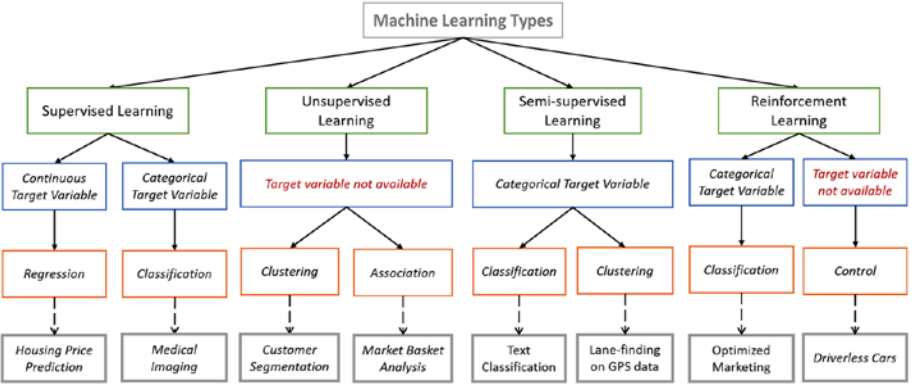
\includegraphics[width=\textwidth]{images/MachineLearningTypes_all}}
\caption{Machine Learning Types nach \citep[S.~222]{ramasubramanian_machine_2017}}
\label{fig:MachineLearningTypes_all}
\end{figure}

\begin{table}[H] \centering
\tiny
\begin{tabular}{|l|l|}
\hline
\textbf{Gruppe} & \textbf{Algorithmen}\\ 
\hhline{==}
Regression Analysis & Ordinary Least Square Regression (OLSR)\\
& Linear Regression\\
& Logistic Regression\\
& Stepwise Regression\\
& Polynomial Regression\\
& Locally Estimated Scatterplot Smoothing (LOESS)\\
\hline
Distance-based algorithms & k-nearest Neighbor (kNN)\\
& Learning Vector Quantization (LVQ)\\
& Self-Organizing Map (SOM)\\
\hline
Regularization algorithms & Ridge Regression\\
& Least Absolute Shrinkage and Selector Operator (LASSO)\\
& Elastic Net\\
& Least-Angle Regression (LARS)\\
\hline
Decision tree algorithms & Classification and Regression Tree (CART)\\
& Iterative Dichotomiser 3 (ID3)\\
& C4.5 and C5.0 (different versions of a powerful approach)\\
& Chi-squared Automatic Interaction Detection (CHAID)\\
& Random Forest\\
& Conditional Decision Tree\\
\hline
Bayesian algorithms & Naive Bayes\\
& Gaussian Naive Bayes\\
& Multinomial Naive Bayes\\
& Nayesian Belief Network (BNN)\\
& Bayesian Network (BN)\\
\hline
Clustering algorithms & k-Means\\
& k-Medians\\
& Partitioning Around Medoids (PAM)\\
& Hierarchical Clustering\\
\hline
Association rule mining & Apriori algorithm\\
& Eclat algorithm\\
& FP-growth algorithm\\
& Context Based Rule Mining\\
\hline
Artificial neural networks & Perception\\
& Back-Propagation\\
& Hopfield Network\\
& Radial Basis Function Network (RBFN)\\
\hline
Deep learning algorithms & Beep Boltzmann Machine (DBM)\\
& Deep Belief Networks (DBN)\\
& Convolutional Neural Network (CNN)\\
& Stacked Auto-Encoders\\
\hline
Dimensionality reduction algorithms & Principam Component Analysis (PCA)\\
& Principam Component Regression (PCR)\\
& Partial Least Squares Regression (PLSR)\\
& Multidimensional Scaling (MDS)\\
& Linear Discriminant Analysis (LDA)\\
& Mixture Discriminant Analysis (MDA)\\
& Quadratic Discriminant Analysis (QDA)\\
\hline
Ensemble learning & Boosting\\
& Bagging\\
& AdaBoost\\
& Stacked Generalization (blending)\\
& Gradient Boost Machines (GBM)\\
\hline
Text mining algorithms & Automatic summarization\\
& Named entity recognition (NER)\\
& Optical character recognition (OCR)\\
& Part-of-speech tagging\\
& Sentiment analysis\\
& Speec recognition\\
& Topic Modeling\\
   \hline
\end{tabular}
\caption{Sebjective Grouping nach \citep[S.~224-229]{ramasubramanian_machine_2017}}
\label{tab:SebjectiveGrouping}
\end{table}

Da der Artikel "How to choose algorithms for Microsoft Azure Machine Learning" von \citep{ericson_microsoft_2017} nach "Supervised", "Unsupervised" und "Reinforcement learning" zurückgreift, wird nachfolgend diese Gliederung genutzt und um "Semi-supervised Learning" und "Active Learning" erweitert. \par

\section{Supervised Learning}\label{subsec:sl}
Die möglicherweise am einfachsten nachvollziehbare Gruppe des Machine Learning ist das Supervised Learning, da es "sehr ähnlich zu dem Prozess ist, in dem Menschen Dinge lernen"\citep[S.~13; eigene Übersetzung]{kim_matlab_2017}. Es existiert ein Datensatz, bei dem für jeden Input ein Output vorhanden ist. Ein Beispiel können Patientendaten sein, die als Output eine Variable besitzen, die angibt, ob ein Patient an Krebs erkrankt ist oder nicht \citep[S.~222]{ramasubramanian_machine_2017}. Diese "response variable" (Krebs oder nicht Krebs) wird als "label"\citep[S.~222]{ramasubramanian_machine_2017} bezeichnet. Die Aufgabe des Learning Prozesses ist es dann, einen Zusammenhang zwischen dem Input (Patientendaten) und dem Label (Krebs oder nicht Krebs) herzustellen. Dies geschieht mit sogenannten "training sets"\citep[S.~5]{paluszek_matlab_2017}. Der zweite Schritt ist dann das Überprüfen des entstandenen Models. Dabei wird das Model auf ein zweites gelabeltes "test set"\citep[S.~5]{paluszek_matlab_2017} angewandt und das Ergebnis überprüft.\par
Die Algorithmen des Supervised Learning lassen sich erneut aufteilen:

\subsection{Classification} \label{subsubsec:classification}
Betrachtet man die Labels und stellt fest, dass sie die Datensätze in Kategorien unterteilen (Krebs oder nicht Krebs) oder eine Wahrscheinlichkeit angeben (Person ist zu 89\% Max Mustermann bei einer Gesichtserkennung), handelt es sich um eine Klassifikation (engl. Classification) \citep[S.~67]{swamynathan_mastering_2017}. Kauchak nennt als Beispiele
\begin{itemize}
\item biometrische Erkennungen (Gesicht, Iris, Unterschrift etc.),
\item Buchstabenerkennung,
\item Spamfilter und
\item medizinische Diagnosen \citep[S.~5]{kauchak_neural_2016}.
\end{itemize}
Weiterhin kann zwischen Klassifikationen mit nur zwei Labels ("two-class or binomial classification"\citep{ericson_how_2017}) (siehe Abbildung \ref{fig:classification}) oder mehr als zwei Labels ("multi-class classification"\citep{ericson_how_2017}) unterschieden werden.
\begin{figure}[H]
\centering
\frame{
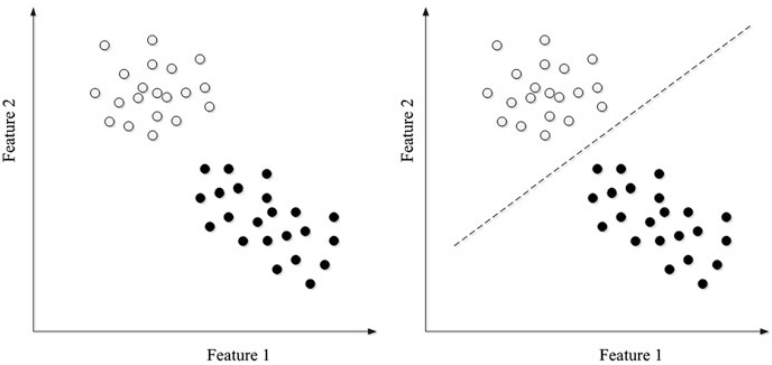
\includegraphics[width=\textwidth]{images/classification}}
\caption{Beispiel für eine Binomialklassifikation aus \citep[S.~8]{suthaharan_machine_2016}}
\label{fig:classification}
\end{figure}

\subsection{Regression}\label{subsubsec:regression}
Wenn eine Unterteilung in Kategorien, wie gerade genannt, nicht möglich ist und die Outputvariable ein fortlaufender Wert (engl. continuous value) ist, werden Regressionen herangezogen. Dabei liegt der "Hauptfokus [...] darin, einen Zusammenhang zwischen einer abhängigen Variablen und einer oder mehreren unabhängigen [...] Variablen herzustellen"\citep[S.~60; eigene Übersetzung]{swamynathan_mastering_2017}. Neben dem bekanntesten Beispiel
\begin{itemize}
\item einen Kurs an der Börse vorherzusagen \multicitep{kauchak_neural_2016, S.~5; kubat_introduction_2017, S.~207; ericson_how_2017}, gibt es Anwendungsfälle in
\item der Epidemiologie,
\item der Auto- und Flugzeugnavigation und
\item Analysen im zeitlichen Verlauf (Wetterveränderung im Verlauf der Zeit)\citep[S.~5]{kauchak_neural_2016}.
\end{itemize}

\subsection{Anomaly detection}
Im bereits mehrfach zitierten Artikel "How to choose algorithms for Microsoft Azure Machine Learning" von \citep{ericson_how_2017} wird noch eine zusätzliche Kategorie genannt: Anomaly detection. Bei \citep[S.~68]{swamynathan_mastering_2017} ist die Anomaly detection dem Unsupervised Learning zugeordnet. Dies rührt daher, dass es darauf ankommt, ob eine Outputvariable ("Label") vorhanden ist, oder nicht. Tatsächlich ist es so, dass es sowohl Szenarien für Supervised und Unsupervised Anomaly detection gibt, als auch für das später noch beschriebene Semi-supervised Learning \citep[S.~15:10]{chandola_anomaly_2009}.
Unabhängig davon beschreibt Anomaly detection das Finden von Mustern in Daten, die vom erwarteten Verhalten abweichen. Diese Pattern werden meist als Anomalie (engl. anomaly) oder Ausreißer (engl. outliner) bezeichnet \citep[S.~15:1]{chandola_anomaly_2009}.
Die Anomaly detection kann für folgende Szenarien genutzt werden\citep[S.~15:2]{chandola_anomaly_2009}:
\begin{itemize}
\item Kreditkartenbetrugserkennung
\item Versicherungsbetrugserkennung
\item Gesundheitsprüfungen
\item Intrusion Detection
\item Militärische Überwachungen
\item Anwendungen in "der Welt des Internet der Dinge"[S.~68]\citep{swamynathan_mastering_2017}
\end{itemize}

\section{Unsupervised Learning}\label{sec:us1}
Der 'Glücksfall', dass der vorhandene Datensatz Label besitzt, tritt unter realen Umständen selten auf. Um aus diesen Daten trotzdem Schlüsse zu ziehen, werden Methoden des Unsupervised Learning herangezogen. Hier liegt der Fokus auf dem "Entdecken von aufschlussreichen Eigenschaften der verfügbaren Daten"\citep[S.277; eigene Übersetzung]{kubat_introduction_2017} und der "Untersuchung der Charakteristik der Daten"\citep[S.~13; eigene Übersetzung]{kim_matlab_2017}. Dies kann das Ziel haben, komplexe und vielschichtige Daten zu vereinfachen und zu strukturieren\citep{ericson_how_2017} oder die Daten in Gruppen aufzuteilen\citep[S.~22]{lison_introduction_2012}. Um diese Gruppen ähnlicher Daten - sogenannte Cluster - geht es im nächsten Abschnitt.\par
Supervised Learning findet man nach \citep[S.~223]{ramasubramanian_machine_2017}
\begin{itemize}
\item bei der Aufteilung von Kundendaten in Segmente,
\item in Analysen von sozialen Netzwerken,
\item in der Klimatologie,
\item bei der Bildkompression und
\item in der Bioinformatik \citep[S.~6]{kauchak_neural_2016}.
\end{itemize}

\subsection{Clustering}
Beim angesprochenen Clustering handelt es sich um das "Identifizieren von distinkten Gruppen [...] basierend auf irgendeiner Art der Ähnlichkeit innerhalb des vorliegenden Datensatzes"\citep[S.~195; eigene Übersetzung]{swamynathan_mastering_2017}. Damit die Objekte der gebildeten Cluster "aussagekräftig und sinnvoll" sind, sollen "die Objekte innerhalb eines Clusters [...] homogen sein" und "zu Objekten anderer Cluster"\citep[S.~337; eigene Übersetzung]{ramasubramanian_machine_2017} heterogen (siehe Abbildung \ref{fig:clustering}). Es kann jedoch auch sein, dass Objekte zu mehreren Clustern gehören. Dies nennt sich "Soft Clustering" - im Gegensatz zum "Hard Clustering"\citep[S.~339]{ramasubramanian_machine_2017}. Die Metrik für die Ähnlichkeit ist nicht festgelegt. Möglich sind 
\begin{itemize}
\item die "Distanz [...] zwischen Beobachtungen", 
\item die "Entfernung vom Mittelwert jeder Beobachtung/des Clusters",
\item die "Signifikanz [einer] statistischen Verteilung" oder
\item die "Dichte im Datenraum"\citep[S.~338; eigene Übersetzung]{ramasubramanian_machine_2017}.
\end{itemize}
\begin{figure}[H]
\centering
\frame{
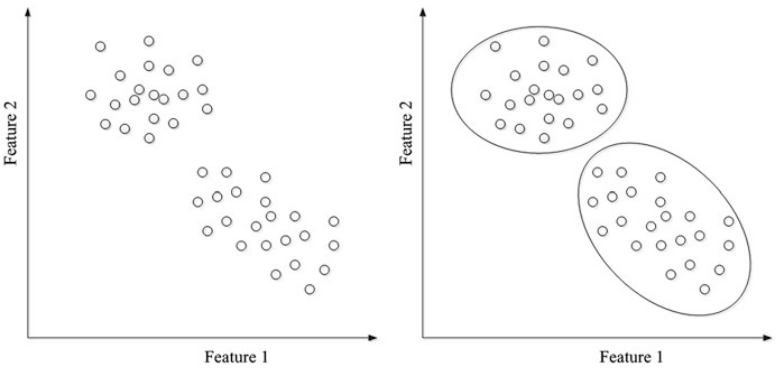
\includegraphics[width=\textwidth]{images/clustering}}
\caption{Beispiel für zwei Cluster \citep[S.~9]{suthaharan_machine_2016}}
\label{fig:clustering}
\end{figure}

\section{Semi-supervised Learning}\label{sec:ssl1}
Bis jetzt wurden zwei Extremfälle beschrieben: entweder es gibt keine Labels oder alle Daten sind gelabelt. Es existieren jedoch auch Abstufungen dazwischen. Besitzen die meisten Daten ein Label, so ist es eventuell möglich, die Datensätze ohne Label für das Learning zu entfernen und ein Model aus dem Supervised Learning heranzuziehen. Tritt aber ein Problem auf, bei dem nur sehr wenige Daten gelabelt sind, empfiehlt sich ein Vorgehen aus dem Semi-supervised Learning. Methoden dieser Familie des Machine Learning beruhen auf der Annahme, dass "die Daten wichtige Informationen über die Gruppenzugehörigkeit beinhalten", "obwohl die Gruppenzugehörigkeit [...] unbekannt ist"\citep[S.~223; eigene Übersetzung]{ramasubramanian_machine_2017}. Als umfassendes Werk für Semi-supervised Learning ist an dieser Stelle \citep{chapelle_semi-supervised_2006} zu nennen. \par
Zur Anwendung kommt Semi-supervised Learning seit den 1990er Jahre in "natural language problems" und "text classification"\citep[S.~4]{chapelle_semi-supervised_2006}.

\section{Active Learning}\label{sec:al1}
Ein Sonderfall des Semi-Supervised Learning ist das Active Learning. Hier wird davon ausgegangen, dass nur wenige oder keine Labels vorhanden sind, diese jedoch durch einen "Menschen mit umfangreichem Wissen im Themengebiet"\citep[S.~i; eigene Übersetzung]{olsson_literature_2009} hinzugefügt werden können. Alle Daten mit einem Label zu versehen wäre jedoch zu "schwer, zeitaufwendig oder zu teuer"\citep[Abstract; eigene Übersetzung]{settles_active_2010}. Mit dem Ziel an den Menschen nur so wenig Anfragen (engl. Queries) wie nötig zu stellen\citep[Abstract]{olsson_literature_2009}, werden Algorithmen entworfen, die selbst wählen können, welche Datensätze gelabelt werden sollen \citep[Abstract]{settles_active_2010}.\par
Nach \citep[S.~4]{settles_active_2010} wird Active Learning beispielsweise in
\begin{itemize}
\item der Spracherkennung,
\item der Informationsextraktion oder in
\item der Klassifikation oder dem Filtern von Dokumenten oder Mediendateien eingesetzt.
\end{itemize}

\section{Reinforcement Learning}\label{sec:rl1}
"Beim Reinforcement Learning interagiert der Lerner" - also ein Programm - "mit seiner Umwelt"\citep[S.~45; eigene Übersetzung]{settles_active_2010}. Er "experimentiert" dabei, um eine Lösung auf das gestellte Problem zu finden und erhält je nach Ausgang seiner Aktion eine Belohnung oder eine Bestrafung \citep[S.~331]{kubat_introduction_2017}. Es wird also nicht direkt mit einem Output (Label) gearbeitet, sondern lediglich die Qualität des Outputs bewertet. Das Ziel ist, durch ein iteratives Vorgehen (siehe Abbildung \ref{fig:reinforcementLearning}), ein maximales Endergebnis (größter Reward) zu erreichen \citep[S.~69]{swamynathan_mastering_2017}.
\begin{figure}[H]
\centering
\frame{
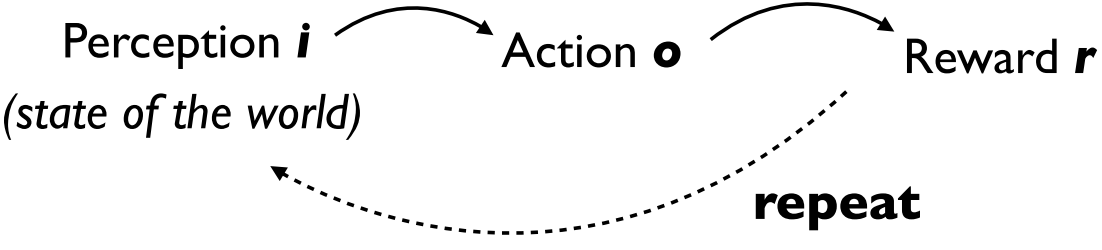
\includegraphics[width=12cm]{images/reinforcementLearning}}
\caption{Iterativer Reinforcement Learning Prozess aus \citep[S.~25]{lison_introduction_2012}}
\label{fig:reinforcementLearning}
\end{figure}
Reinforcement Learning kommt in Szenarien zum Einsatz, in denen noch keine Daten zum Lernen zur Verfügung stehen oder erst nach und nach aktualisiert werden \citep[S.~223]{ramasubramanian_machine_2017}.\par
Ein prominentes Beispiel für ein System mit Reinforcement Learning ist Google DeepMinds AlphaGo. Es handelt sich dabei um ein Go (asiatisches Brettspiel) spielendes Computersystem, das seine Spielstärke durch spielen gegen sich selbst erreichte \citep{silver_mastering_2017}. AlphaGo besiegte 2015 den "legendären Mr Lee Sedol" (weitgehend als bester Spieler des Jahrzehnts geachtet) vor 200 Millionen Zuschauern \citep{deepmind_alphago_2017}.

\chapter{Kryptowährungen}\label{sec:cryptocurrency2}
In der Motivation (siehe Abschnitt \ref{sec:cryptocurrency}) wurde bereits auf Kryptowährungen allgemein und auf Bitcoin im Speziellen eingegangen. Es wurde ebenfalls angemerkt, dass die zwei Währungen mit dem größten Marktvolumen Bitcoin (\gls{btc}) und Etherium (\gls{eth}) sind. Aus diesem Grund werden die Kurse dieser beiden Währungen analysiert. In diesem Abschnitt wird darauf verzichtet, weiter auf die allgemeine Technik hinter BTC und ETH einzugehen. In Punkt \ref{subsec:describe} - vor allem in den Tabellen \ref{tab:BTCextraData} und \ref{tab:ETHextraData} - tauchen bei der Beschreibung der Datensätze jedoch Begriffe auf, die einer genaueren Erklärung bedürfen:
\begin{itemize}
\item Die \textbf{Marktkapitalisierung} ist der aktuelle Marktwert einer Kryptowährung. Er ergibt sich aus dem Produkt des aktuellen Handelskurses und der totalen Anzahl der geschürften Währungseinheiten. Bei einem Kurs von 500 USD pro \gls{ether} und einem Volumen von 1000 Ether, ist die Marktkapitalisierung 500000 USD.
\item Das Handelsvolumen (engl. \textbf{trade volume}) ist die Anzahl der Kryptowährungseinheiten, die in einem bestimmten Zeitfenster - meist 24 Stunden - gehandelt wurden.
\item Die \textbf{Blocksize} ist die Größe eines Blocks (meinst in Megabyte).
\item \textbf{Stale Blocks} sind Blöcke der Blockchain, die korrekt sind, aber ihren Weg in die Blockchain nicht gefunden haben. Dies kann passieren, wenn zwei Blöcke gleichzeitig fertiggestellt werden, jedoch nur einer davon in die Blockchain aufgenommen werden kann \citep{bitcoinproject_stale_2017}. Im Ethereumnetzwerk heißen diese Blöcke '\textbf{Uncles}'. Entgegen dem Bitcoinnetzwerk werden dort Miner für Stale Blocks (Uncles) entlohnt \citep{jdebunt_what_2017}. Es besteht auch die Möglichkeit eines '\textbf{Orphaned}' Blocks. Das ist ein Block, über dessen Elternblöcke ein berechnender Knoten des Netzwerks keine Informationen hat und ihn deswegen nicht validieren kann \citep{bitcoinproject_orphan_2017}.
\item Die Bestätigungszeit (engl. \textbf{confirmation time}) ist die Zeit, die zwischen einer Transaktion und ihrer Aufnahme in die Blockchain vergeht \citep{kumar_cryptocurrency_2017}.
\item Bei der \textbf{Hashrate} handelt es sich um die Anzahl der Hashes eines Netzwerks pro Sekunde. Trifft man auf den Begriff im Kontext des Bitcoins, handelt es sich meist um Terahashes, bei Ethereum um Gigahashes (entspricht $ \frac{1}{1000}$ Terahash) \citep{kumar_cryptocurrency_2017}.
\item Miningschwierigkeit (\textbf{difficulty}) meint die Schwierigkeit, einen validen Block zu finden. Als Referenz dient die einfachste Möglichkeit einen Block zu finden mit der Schwierigkeit 1 \citep{bitcoinproject_difficulty_2017}.
\item Aufgebrachte Rechenleistung wird im Ethereumnetzwerk in \textbf{Gas} (engl. Aussprache) bemessen. Wie in Teil \ref{sec:cryptocurrency} bereits genannt, können im Netzwerk beispielsweise Smartcontracts ausgeführt werden. Die Kosten für die dort verbrauchte Leistung wird in Gas gezahlt. Wenn die Leistung vorher nicht abgemessen werden kann, wird ein Limit (\textbf{gas limit}) gesetzt, nach dessen Verbrauch eine Aktion abgebrochen wird \citep[S.~4]{wood_ethereum:_2014}.
\end{itemize}

\chapter{Microsoft Azure ML Studio}\label{sec:msmls}
Im nun folgenden Abschnitt der Arbeit wird das Microsoft Azure ML Studio in drei Schritten erklärt:
\begin{enumerate}
\item Zuerst erfolgt eine allgemeine Beschreibung des Machine Learning Studios.
\item Dann wird der Aufbau eines Projektes beschrieben und
\item zuletzt die vorgefertigten Komponenten vorgestellt.
\end{enumerate}
Es sollte in diesem Teil beachtet werden, dass die Quellen hauptsächlich Microsoft-eigen sind, da außer einigen Blogartikeln wenig externe Literatur oder Meinungen verfügbar sind.
\section{Allgemeine Beschreibung}\label{sec:ab1}
Zum Ende des Abschnittes \ref{sec:SaaS} wurde die \textbf{S}oftware \textbf{a}s \textbf{a} \textbf{S}ervice (SaaS) Microsoft Azure Machine Learning Studio bereits angesprochen. Es handelt sich dabei um eine Cloud-basierte Web-\gls{ide} (\textbf{I}ntegrated \textbf{D}evelopment \textbf{E}nvironment). Der Kern der Anwendung ist ein "drag and-drop tool", das genutzt wird, um "predictive analytics solutions" zu entwerfen und bereitzustellen \citep{ericson_what_2017}. Es können sowohl vorgefertigte Bausteine genutzt werden, als auch selbst entworfene Scripte (in \gls{r} und/oder \gls{py}).
\section{Aufbau und Komponenten}\label{sec:auK1}
Die strukturellen Hauptkomponenten sind Tabelle \ref{tab:azuremlcomponents} zu entnehmen. Die Tabelle basiert auf dem Artikel "What is Azure Machine Learning Studio?" von \citep{ericson_what_2017} und dem Machine Learning Studio selbst (https://studio.azureml.net/Home).
\begin{longtable}[H]{|p{2,5cm}|p{14cm}|}
\hline
\textbf{Komponente} & \textbf{Beschreibung}\\ 
\hhline{==}
Settings & Hier finden sich Einstellmöglichkeiten zur Benutzerverwaltung (für kollaborative Arbeit im Studio), das Preismodell (10GB Workspace Storage sind in der kostenfreien Version enthalten) und die Authorisierungstoken. Die Settings sind in diesem Kontext nicht weiter interessant. \\
\hline
Notebooks & Die Notebooks sind Verknüpfungen auf Jupyter Notebooks. Diese wiederum sind "Webanwendungen", die genutzt werden, um "Dokumente, die live code, Gleichungen, Virtualisierungen und erzählenden Text" enthalten "zu erstellen und zu teilen". Genutzt werden sie unter anderem für 
\begin{itemize}
\item "data cleaning",
\item "transformation,
\item numerical simulation,
\item statistical modeling,
\item data visualization" und
\item "machine learning"\citep{projectjupyter_jupyter_2017}.
\end{itemize}
Project Jupyter ist non-profit und open-source \citep{projectjupyter_about_2017}. \\
\hline
Experiments & Experimente sind das Kernelement des Azure ML Studios. Sie stellen den Rahmen für das Erproben verschiedener Problemlösungen. Experimente sollten dabei mindestens ein Datenset (dazu gleich mehr) und ein Modul enthalten. Ist ein Experiment ausgereift, kann der Status von "training" to "predictive" geändert werden und als Web Service bereit gestellt werden (dazu ebenfalls nachfolgend mehr).\\
\hline
Datasets & Für das Experimentieren benötigte Datensätze (z.B. .csv-, .tsv-, .arff-, .txt-, .zip-, oder .RData-Dateine) können in die Web-IDE geladen und als Datasets abgespeichert werden. So können die Dateien ohne erneutes Hochladen wiederverwendet werden. Eine andere Möglichkeit, Daten im Studio zu benutzen, ist das Experiment Item "Import Data", das unter anderem auf Daten aus Azure Blob Storage, Azure Table Storage, Azure DocumentDB, Azure SQL Datenbanken, Hive Queries oder HTTP-Quellen zugreifen kann.\\
\hline
Experiment Items & Die Sammlung aller drag-and-drop Elemente im Studio werden Experiment Items genannt. Sie umfassen Elemente für alle Prozessschritte, wie Input, Transformation, Selection, Machine Learning Module, Visualisierung, Scoring etc.\\
\hline
Trained Models & Fertig trainierte Machine Learning Module können als eigenständige Komponenten genutzt werden. Ein Beispiel dafür wäre die Wiederverwendung in einem anderen Experiment mit neuen Daten oder der Vergleich zweier fertiger Modelle.\\
\hline
Web Services & Ist ein Experiment auf dem Status "predictive", können die Input- und Output-Felder in Web Services umgewandelt werden, um sie in andere Anwendungen oder Systeme zu integrieren.\\
\hline
Projects & Projects dienen als organisatorisches Strukturelement. Durch sie können Experimente, Datasets, Notebooks etc. gruppiert werden. \\
\hline
\caption{Hauptkomponenten des Azure Machine Learning Studios}
\label{tab:azuremlcomponents}
\end{longtable}



\input{parts/Durchführung}

\chapter{Zusammenfassung, Fazit und Ausblick}\label{chap:Bewertung}

\section{Bewertung von Azure Machine Learning Studio}\label{sec:BeswertungAzure}
Bei Azure Machine Learning Studio handelt es sich um ein Werkzeug mit klarer Oberfläche. Das Einlernen und Navigieren zwischen Experimenten und Projekten ist sehr einfach. Die Funktionen sind auf den ersten Blick verständlich. Es bietet die Standardoperationen des Supervised Learning an (Read, Clean, Transform, Split, Train, Tune, Score, Evaluate). Dadurch gelingt es, schnell zu Ergebnissen zu kommen.\par
Das Werkzeug vermittelt den Eindruck, dass nicht viel Hintergrundwissen benötigt wird. Dies stimmt bei genauerem Hinsehen jedoch nicht. Bei der Auswahl der Algorithmen lassen sich alle Algorithmen auswählen, auch, wenn sie nicht zum vorliegenden Problem passen. So lässt sich beispielsweise eine 'Two-Class Bayes Point Machine' auf ein offensichtlich nicht-lineares Problem anwenden. Dies ist kein Fehler des Werkzeugs, es zeigt nur auf, dass nicht auf Hintergrundwissen verzichtet werden kann. Dies fällt auch auf, wenn  das Experiment Item 'Clean Missing Data' genutzt wird: Es muss zwischen acht möglichen Bereinigungsmethoden entschieden werden, zu denen auch Probabilistic PCA und MICE gehören. Allein diese Auswahl erfordert Recherchearbeit.
Andererseits bietet sich auch die Möglichkeit, verschiedene Einstellungen schnell und einfach auszuprobieren und so über 'trial und error' zu lernen.\par
Ein großer Kritikpunkt ist, dass es passieren kann, dass Experimente beim Durchlaufen nicht terminieren. Sie laufen ewig oder werden nach einer Stunde ohne Fehlermeldung beendet. In der Free-Version ist eine parallele Verarbeitung mehrerer Experimente nicht möglich, deswegen führen diese Fehler zum Stillstand.\par
Die Dokumentation ist angemessen und gibt einen guten Überblick über alle Features. An manchen Stellen wäre etwas mehr Information jedoch wünschenswert. Die Untersuchung ist an die Limitation von 100 Experiment Items pro Experiment und die maximale Experimentdauer von einer Stunde gestoßen.\par
Azure Machine Learning bietet nur Supervised Learning an.\par
Grundsätzlich ist der Erweiterbarkeit durch eigene Skripte (Python oder R) keine Grenzen gesetzt, es kann im Tool jedoch kein Debugging durchgeführt werden. Nicht-trivialer Code muss zuvor lokal getestet werden. Ebenfalls gibt es keine Versionsverwaltung, was für Analysten mit Software Engineering Hintergrund sicherlich ein Manko darstellt.\par
Als Fazit kann festgehalten werden, dass Azure Machine Learning Studio ein gutes Werkzeug ist, das alle Grundfunktionen beinhaltet. Es ist gut dokumentiert und gut für Standardprobleme einsetzbar. Es lässt sich einerseits für Vorstudien in Projekten empfehlen, wenn herausgefunden werden muss, ob ein Problem mit den Mitteln des Machine Learning lösbar ist. Andererseits bietet es durch viele integrierte Beispiele einen perfekten Rahmen für das Lernen des Vorgehens beim Machine Learning.

\section{Bewertung des CRISP-DM Referenzmodells}\label{sec:BeswertungCrisp}
Das CRISP-DM Referenzmodell ist ein sehr guter Leitfaden für alle Beteiligten an einem Data Mining Projekt. Vor allem für Analysten mit wenig Erfahrung bietet der User Guide eine große Hilfestellung. Das Modell legt viel Wert auf Dokumentation und Nachvollziehbarkeit. Es versucht, zwischen den betriebswirtschaftlichen, fachlichen und technischen Aspekten zu unterscheiden. Dies gelingt nicht immer ganz. Durch diese Betrachtung aus verschiedenen Blickwinkeln bietet der User Guide viele Tipps und stellt sicher, dass nichts vergessen oder übersehen wird.\par
Empfehlenswert ist eine Anwendung des Modells als roter Faden in Data Mining, Machine Learning und anderen Data Science oder Analytics-Projekten. Es muss nur so abgeändert werden, dass es auf das Problem passt. Da es sehr umfangreich ist, kann - wie in der vorliegenden Arbeit - etwas weggelassen oder hinzugefügt werden.

\section{Bewertung der Ergebnisse des Machine Learning}\label{sec:BewertungML}
Der Analyseansatz in der Arbeit war, mit der Recherche nach Einflussfaktoren zu beginnen. Dabei wurden viele Faktoren ausgewählt. Diese wurden genauer untersucht, ausgedünnt und bearbeitet. Anschließend wurde das Machine Learning durchgeführt. Wenn dieser Ansatz verfolgt wird, ist es empfehlenswert, im Vorfeld bereits einen oder zwei Algorithmen auszuwählen (z.B. 'Two-Class Bayes Point Machine', da er widerstandsfähig gegen Overfitting ist), die genutzt werden sollen. Dadurch kann mehr Zeit aufgewendet werden, die Daten in eine bessere Struktur zu bringen.\par
Mit dem gewonnenen Wissen empfiehlt sich jedoch eher die Auswahl von einem oder zwei Faktoren (z.B. Kurs des Dow Jones (DJIA) und des Goldpreises). Dadurch können mehr Hilfsanalysen (z.B. Auseinanderschneiden (engl. slicing) der Daten und Suchen nach Zusammenhängen in bestimmten Zeitperioden) durchgeführt werden. Auch wird weniger Zeit für das Beschreiben und Zusammenführen der Daten verwendet als für detaillierte Untersuchungen.\par
Es kann festgehalten werden, dass die Arbeit vorherige Untersuchungen unterstreicht, dass der Kursverlauf von Kryptowährungen nicht zufällig ist, sondern mit Faktoren wie dem öffentlichen Interesse (z.B. Google Suchanfragen) zusammenhängt.\par
Auch wenn Tendenzen im Kursverlauf durch Machine Learning aufgedeckt werden können, gibt es zu viele Einflüsse, über die keine Daten vorhanden sind. So wird beispielsweise geschätzt, dass über 50-80\% der Miningpower im Bitcoinnetzwerk von chinesischen Miningpools kontrolliert wird \multicitep{wagenknecht_bitcoin_2016; tuwiner_10_2017}. Die Absprachen dieser Pools können großen Einfluss haben. 
Eine andere Erkenntnis ist, dass die Kurse im Analysezeitraum tendenziell ansteigend waren. Aus diesem Grund besitzen Regressionen einen sehr hohen Wert für $ R^2 $. Eventuell muss hier eine andere Metrik zum Einsatz kommen.\par
Im realen Betrieb eines Systems zur Vorhersage, müsste darauf geachtet werden, dass die zur Analyse verwendeten Daten parallel erhoben werden müssen. So kann sich beispielsweise die Größe "Tageshoch des WTI-Ölpreises" ständig ändern. Außerdem handelt es sich bei BTC und ETH um die wahrscheinlich prominentesten Kryptowährungen. Kleinere Altcoins unterliegen möglicherweise anderen Einflüssen. Auch die Wechselwirkung zwischen den Währungen darf nicht vernachlässigt werden.\par
Zum Schluss muss noch erwähnt werden, dass es sich definitiv um eine sehr komplexe Problemstellung handelt, die eventuell mit Standardvorgehen und -mitteln nicht lösbar ist.


%\bibliographystyle{ieeetran}
%\bibliographystyle{plain}
%\bibliographystyle{apalike}
\bibliographystyle{apa}

\bibliography{Masterarbeit}

\end{document}
